% Informe del Proyecto 2 (Entregable 2) — MiniDB multimodal
% Compilar:  cd docs/informe && tectonic informe_e2.tex   (o latexmk -pdf informe_e2.tex, o Overleaf)
% Las tablas de tablas/exp5*.tex ... exp8.tex y las figuras exp5_*.png ... exp8_*.png se regeneran con:
%   python -m benchmarks.run_all --only 5 6 7 8 && python -m benchmarks.report_tables
\documentclass[11pt,a4paper]{article}

\usepackage{iftex}
\ifPDFTeX
  \usepackage[utf8]{inputenc}
  \usepackage[T1]{fontenc}
  \usepackage{lmodern}
\else
  \usepackage{fontspec}
\fi
\usepackage[spanish,es-noshorthands,es-tabla,es-nodecimaldot]{babel}
\usepackage[margin=2.2cm]{geometry}
\usepackage{amsmath,amssymb}
\usepackage{graphicx}
\usepackage{booktabs}
\usepackage{tabularx}
\usepackage{array}
\usepackage{multirow}
\usepackage{xcolor}
\usepackage{listings}
\usepackage{caption}
\usepackage{subcaption}
\usepackage{float}
\usepackage{enumitem}
\usepackage{tikz}
\usetikzlibrary{positioning,arrows.meta,calc,fit}
\usepackage[hidelinks]{hyperref}

\graphicspath{{figuras/}}
\setlength{\parskip}{0.35em}
\setlist{itemsep=0.15em,topsep=0.3em}
\captionsetup{font=small,labelfont=bf}

\definecolor{codebg}{RGB}{246,248,250}
\definecolor{kw}{RGB}{0,92,197}
\lstdefinestyle{sql}{
  language=SQL, basicstyle=\ttfamily\small, keywordstyle=\color{kw}\bfseries,
  backgroundcolor=\color{codebg}, frame=single, rulecolor=\color{black!15},
  columns=fullflexible, breaklines=true, literate={á}{{\'a}}1 {é}{{\'e}}1 {í}{{\'i}}1 {ó}{{\'o}}1 {ú}{{\'u}}1 {ñ}{{\~n}}1,
  morekeywords={USING,HEAP,SEQUENTIAL,BTREE,HASH,COPY,EXPLAIN,BETWEEN,INDEX,RTREE,INVERTED,IVF,WITH,MATCH,
                WITHIN_RADIUS,WITHIN_BOX,LIMIT,POINT,VECTOR,TEXT,COSINE_SCORE}
}
\lstdefinestyle{txt}{basicstyle=\ttfamily\small, backgroundcolor=\color{codebg}, frame=single,
  rulecolor=\color{black!15}, columns=fullflexible, breaklines=true}
\newcommand{\code}[1]{\texttt{#1}}

\hypersetup{pdftitle={MiniDB multimodal: índices espaciales, textuales y vectoriales en disco},
  pdfauthor={Renzo Acervo, Josué Toribio, Lisseth Rondan}}

\begin{document}

%----------------------------- Portada estilo artículo -----------------------------
\thispagestyle{plain}
\begin{center}
{\LARGE MiniDB multimodal: índices espaciales, textuales y vectoriales en disco\par}
\vspace{1.4em}
{\large Renzo Acervo\textsuperscript{a}, Josué Toribio\textsuperscript{a}, Lisseth Rondan\textsuperscript{a}\par}
\vspace{1em}
{\small\itshape \textsuperscript{a}Departamento de Ciencia de la Computación, Universidad de Ingeniería y
Tecnología (UTEC), Lima, Perú\par}
\vspace{0.5em}
{\small Proyecto 2 (Entregable 2) --- Base de Datos II (CS2042) --- 2026-II --- Docente: Percy Lovon Ramos\par}
\end{center}

\vspace{1.5em}
\noindent\rule{\textwidth}{0.4pt}\par
\vspace{0.4em}
\noindent\textbf{Resumen}\par
\vspace{0.3em}
\noindent Extendimos MiniDB, el motor relacional en disco del Entregable~1, para indexar y consultar
datos no convencionales sin salir de memoria secundaria. Agregamos tres tipos de columna
(\code{POINT}, \code{TEXT} y \code{VECTOR}) y tres índices paginados construidos desde cero: un
\textbf{R-Tree} con división cuadrática, empaquetado STR y búsqueda $k$-NN \emph{best-first}; un
\textbf{índice invertido} separado en diccionario y listas de posteo, construido con SPIMI, con
consultas booleanas por mezcla de dos punteros y ranking TF-IDF con similitud de coseno; y un índice
vectorial aproximado \textbf{IVF-Flat} con directorio de centroides y listas invertidas paginadas. El
parser SQL acepta \code{WITHIN\_RADIUS}, \code{MATCH}, \code{COSINE\_SCORE()}, los operadores
\code{<->} y \code{<=>} y \code{ORDER BY \dots\ LIMIT}, y un planificador híbrido decide entre
\emph{pre-filtering} y \emph{post-filtering} e informa los bloques leídos en el índice y en la tabla.
Sobre el motor desplegamos un \textbf{recomendador multimodal de productos de moda} (44\,072
productos con imagen) que compara, en vivo, \emph{Bag of Visual Words} (SIFT + índice invertido)
frente a \emph{embeddings} densos (ResNet-18 + IVF), con filtros de precio (B$^+$) y de cercanía
(R-Tree). Los cuatro experimentos pedidos muestran que el R-Tree resuelve un $k$-NN en 2D leyendo
12%
 bloques frente a 1\,235%
 del recorrido
secuencial pero pierde desde $D\approx16$; que el índice invertido responde consultas booleanas y de
ranking leyendo cientos de bloques frente a miles del \emph{full scan}; que los embeddings superan al
BoVW (Precision@10 de 0.79 frente a 0.51); y que el IVF alcanza 98.6%
\,\% de Recall@10 leyendo
1.6%
\,\% de los bloques del $k$-NN exacto.
\par
\vspace{0.4em}
\noindent\textbf{Palabras clave:} R-Tree, índice invertido, SPIMI, TF-IDF, IVF, búsqueda aproximada de
vecinos, \emph{filter-and-refine}, planificación híbrida.
\par\vspace{0.2em}
\noindent\rule{\textwidth}{0.4pt}

\vspace{0.6em}
\tableofcontents
\newpage

%==========================================================================================
\section{Introducción}

El Entregable~1 dejó un motor relacional que opera sobre archivos binarios paginados: toda página se
transfiere con \code{seek} + \code{read}/\code{write}, se serializa con \code{struct} y cada
transferencia la cuenta el \code{DiskCounter}. En este entregable ese mismo motor aprende a indexar
geometrías, texto libre y vectores de alta dimensión, y sirve de base a una aplicación de inteligencia
artificial. El criterio de diseño no cambia: \textbf{toda estructura vive en disco, en páginas de
4\,KB, y cada consulta informa exactamente cuántos bloques leyó}.

\begin{table}[H]
\centering\small
\begin{tabularx}{\textwidth}{@{}lX@{}}
\toprule
Requisito del enunciado & Implementación \\
\midrule
Módulo espacial (R-Tree, radio, $k$-NN, mapa) & \code{backend/indexes/rtree.py}; visor Leaflet en el cliente (sección~\ref{sec:rtree}) \\
Índice invertido en disco, booleano y TF-IDF + coseno & \code{backend/indexes/inverted\_index.py}, \code{backend/text/} (sección~\ref{sec:texto}) \\
BoVW y embeddings; $k$-NN exacto; ANN en disco & \code{backend/ml/features.py}, \code{backend/indexes/ivf.py} (sección~\ref{sec:vector}) \\
Gramática SQL extendida y planificador híbrido & \code{backend/sql/parser.py}, \code{backend/sql/multimodal.py} (sección~\ref{sec:sql}) \\
Aplicación de IA (Opción B: recomendador) & \code{backend/app/recommender.py}, pestaña \emph{Recomendador} (sección~\ref{sec:app}) \\
Experimentos 5 a 8 & \code{benchmarks/exp5\_spatial.py} \dots\ \code{exp8\_ann.py} (sección~\ref{sec:experimentos}) \\
\bottomrule
\end{tabularx}
\caption{Alcance del Entregable~2.}
\end{table}

\paragraph{Restricciones.} Se mantienen las del Entregable~1: sin motores de bases de datos ni ORM,
sin \code{pickle}/\code{json} para persistir, sin leer archivos completos y sin \code{mmap}; todo
acceso a disco pasa por \code{DiskManager}. PostgreSQL aparece únicamente como sistema de referencia
en el Experimento~6. Para la aritmética sobre los bytes de una página ya leída (áreas de cajas,
distancias, K-Means) usamos \code{numpy}: no interviene en el almacenamiento, que sigue siendo una
página por transferencia. Las redes preentrenadas (ResNet-18) y SIFT solo extraen características;
la indexación y la búsqueda son nuestras.

%==========================================================================================
\section{Arquitectura}

\begin{figure}[H]
\centering
\begin{tikzpicture}[
  box/.style={draw, rounded corners=2pt, minimum height=0.8cm, align=center, font=\scriptsize, fill=white},
  wide/.style={box, minimum width=15.4cm},
  arr/.style={-{Stealth[length=2mm]}, thick}]
\node[wide, fill=blue!6] (web) {Cliente web (React): cliente SQL de 4 paneles $\cdot$ visor de mapa (Leaflet) $\cdot$ miniaturas $\cdot$ pestaña \emph{Recomendador}};
\node[wide, below=0.4cm of web, fill=blue!3] (api) {API REST (FastAPI): \code{/api/query} $\cdot$ \code{/api/tables} $\cdot$ \code{/api/app/recommend} $\cdot$ \code{/api/media}};
\node[box, minimum width=3.6cm, below left=0.45cm and -3.6cm of api, fill=purple!6] (app) {Recomendador\\(arma SQL por método)};
\node[box, minimum width=3.6cm, right=0.33cm of app, fill=purple!6] (ml) {Extracción\\ResNet-18 + PCA $\cdot$ SIFT + BoVW};
\node[box, minimum width=3.6cm, right=0.33cm of ml] (parser) {Lexer + Parser\\(gramática extendida)};
\node[box, minimum width=3.6cm, right=0.33cm of parser] (plan) {Planner híbrido + Executor\\(pre / post-filtering)};
\node[box, minimum width=2.25cm, below=0.9cm of app.south west, anchor=north west, fill=orange!8] (heap) {Heap / Sequential\\POINT, TEXT, VECTOR};
\node[box, minimum width=2.25cm, right=0.25cm of heap, fill=green!8] (bt) {B$^+$ $\cdot$ Hash};
\node[box, minimum width=2.25cm, right=0.25cm of bt, fill=green!14] (rt) {R-Tree\\\code{.rtr}};
\node[box, minimum width=3.6cm, right=0.25cm of rt, fill=green!14] (inv) {Índice invertido\\\code{.vocab.dic} \code{.postings.inv} \code{.docs.bin}};
\node[box, minimum width=3.6cm, right=0.25cm of inv, fill=green!14] (ivf) {IVF-Flat\\\code{.ivf.dir} \code{.ivf.lst}};
\node[wide, below=0.45cm of rt.south, xshift=1.55cm, fill=gray!10] (dm) {\code{DiskManager}: \code{seek(page\_id $\cdot$ B)} + \code{read/write(B)} $\cdot$ \code{DiskCounter} total y por archivo};
\draw[arr] (web) -- (api);
\draw[arr] (api.south -| app) -- (app);
\draw[arr] (api.south -| parser) -- (parser);
\draw[arr] (app) -- (ml);
\draw[arr] (parser) -- (plan);
\draw[arr] (app.south) -- ++(0,-0.25) -| ([xshift=-1.2cm]plan.south);
\draw[arr] (plan.south) -- ++(0,-0.45) -| (ivf.north);
\draw[arr] (plan.south) -- ++(0,-0.45) -| (inv.north);
\draw[arr] (plan.south) -- ++(0,-0.45) -| (rt.north);
\draw[arr] (plan.south) -- ++(0,-0.45) -| (bt.north);
\draw[arr] (plan.south) -- ++(0,-0.45) -| (heap.north);
\draw[arr] (rt.south) -- (rt.south |- dm.north);
\end{tikzpicture}
\caption{Capas de MiniDB tras el Entregable~2. En verde oscuro, los índices nuevos; en morado, la
aplicación de IA, que solo habla con el motor a través de sentencias SQL.}
\label{fig:arq}
\end{figure}

La figura~\ref{fig:arq} resume los cambios. El \code{DiskCounter} ahora lleva, además del total, el
\textbf{desglose por archivo}: al terminar cada sentencia \code{Database.execute} clasifica cada
archivo como tabla de datos o índice y devuelve \code{index\_reads} y \code{table\_reads}, que es lo
que el enunciado pide mostrar en las consultas híbridas. La clase \code{Table} mantiene los cinco
tipos de índice con la misma interfaz (\code{insert}, \code{delete}, \code{flush}); el catálogo
binario guarda el tipo de índice y sus opciones (\code{WITH (\dots)}).

\subsection{Tipos de columna nuevos}

El registro sigue siendo de \textbf{longitud fija con bitmap de presencia}; los tipos nuevos ocupan
un campo de bytes de tamaño fijo dentro del registro:

\begin{table}[H]
\centering\small
\begin{tabular}{@{}llll@{}}
\toprule
Tipo & Formato \code{struct} & Bytes & Uso \\
\midrule
\code{POINT} & \code{'dd'} & 16 & coordenadas $(x, y)$ = (longitud, latitud) \\
\code{VECTOR(n)} & \code{'\{n\}f'} & $4n$ & $n$ componentes \code{float32} \\
\code{TEXT(n)} / \code{CHAR(n)} & \code{'\{n\}s'} & $n \le 4000$ & UTF-8 rellenado con \code{\textbackslash x00} \\
\bottomrule
\end{tabular}
\caption{Tipos agregados. Un registro debe caber en una página.}
\end{table}

La tabla de la aplicación, \code{productos(id, titulo, categoria, tipo, genero, color, precio,
tienda, ubicacion POINT, descripcion TEXT(200), imagen, palabras TEXT(800), embedding VECTOR(128))},
tiene registros de 1\,708 bytes: entran 2 por página y sus 44\,072 filas ocupan $P=22\,036$ páginas
(86\,MB). Ese es el costo de cualquier recorrido secuencial sobre ella.

%==========================================================================================
\section{Módulo espacial: R-Tree en disco}
\label{sec:rtree}

\subsection{Diseño físico}

\begin{figure}[H]
\centering
\begin{tikzpicture}[cell/.style={draw, minimum height=0.7cm, font=\scriptsize, align=center}, x=1cm]
\node[cell, minimum width=2.6cm, fill=gray!15] (h) {header 24 B\\\code{record\_count}=$n$};
\node[cell, minimum width=3.4cm, right=0cm of h, fill=green!10] (e1) {$x_{\min}$ $y_{\min}$ $x_{\max}$ $y_{\max}$\\MBR$_1$ = 32 B};
\node[cell, minimum width=1.7cm, right=0cm of e1, fill=orange!14] (p1) {RID$_1$\\6 B};
\node[cell, minimum width=3.4cm, right=0cm of p1, fill=green!10] (e2) {MBR$_2$\\32 B};
\node[cell, minimum width=1.7cm, right=0cm of e2, fill=orange!14] (p2) {RID$_2$\\6 B};
\node[cell, minimum width=1.4cm, right=0cm of p2] (dots) {$\cdots$};
\node[font=\scriptsize, below=0.15cm of e2] {hoja (\code{RTREE\_LEAF}): 107 entradas de 38 B con $B=4096$};
\node[cell, minimum width=2.6cm, fill=gray!15, below=1.15cm of h] (h2) {header 24 B};
\node[cell, minimum width=3.4cm, right=0cm of h2, fill=green!10] (f1) {MBR$_1$ (recubre al hijo)\\32 B};
\node[cell, minimum width=1.7cm, right=0cm of f1, fill=blue!10] (c1) {hijo$_1$\\4 B};
\node[cell, minimum width=3.4cm, right=0cm of c1, fill=green!10] (f2) {MBR$_2$\\32 B};
\node[cell, minimum width=1.7cm, right=0cm of f2, fill=blue!10] (c2) {hijo$_2$\\4 B};
\node[cell, minimum width=1.4cm, right=0cm of c2] {$\cdots$};
\node[font=\scriptsize, below=0.15cm of f2] {nodo interno (\code{RTREE\_INTERNAL}): 113 entradas de 36 B};
\end{tikzpicture}
\caption{Páginas del archivo \code{<tabla>\_<col>.rtr}. La página~0 guarda la raíz, la altura, la
dimensión, el tipo de coordenada, las capacidades y el número de entradas.}
\label{fig:rtree-pag}
\end{figure}

Cada objeto o subárbol se aproxima con su caja envolvente mínima $\text{MBR}=\langle x_{\min},
y_{\min}, x_{\max}, y_{\max}\rangle$ (para un punto, una caja degenerada). El árbol es genérico en la
dimensión $D$ y en el tipo de coordenada ($c=8$ bytes en \code{float64} para coordenadas geográficas,
$c=4$ en \code{float32} para el experimento de dimensionalidad); las capacidades se calculan siempre
desde $B$:
\[
L=\left\lfloor\frac{B-24}{2Dc+6}\right\rfloor,\qquad
M=\left\lfloor\frac{B-24}{2Dc+4}\right\rfloor .
\]
Con $B=4096$ y $D=2$ entran $L=107$ entradas por hoja y $M=113$ por nodo interno; con $D=128$ en
\code{float32} entran solo 3 (tabla~\ref{tab:exp5dim}).

\subsection{Operaciones}

\begin{itemize}
\item \textbf{Inserción.} Se desciende desde la raíz eligiendo en cada nodo la entrada cuya caja
  necesita la \emph{menor ampliación de área} para cubrir el objeto nuevo ($\Delta$Área; en empates,
  la de menor área y luego la de menor margen). El camino se guarda en una pila porque los nodos no
  tienen puntero al padre. Si la hoja tiene espacio se escribe (1W) y solo se reescriben los ancestros
  cuya caja tuvo que crecer.
\item \textbf{División cuadrática} (Guttman). Si la página desborda, \code{PickSeeds} elige el par de
  entradas que desperdiciaría más área al quedar juntas, y \code{PickNext} asigna las demás, una a la
  vez, al grupo cuya caja crece menos, empezando por la entrada con mayor preferencia por un grupo.
  Se garantiza un llenado mínimo del 40\,\%. El ajuste de cajas y los posibles \emph{splits} se
  propagan hacia la raíz; si la raíz se divide, el árbol crece un nivel.
\item \textbf{Carga masiva STR} (\emph{Sort-Tile-Recursive}). \code{CREATE INDEX} sobre una tabla con
  datos ordena los puntos por $x$, los corta en $\lceil\sqrt{N/L}\rceil$ franjas y dentro de cada
  franja los ordena por $y$; cada grupo de $L$ puntos es una hoja, y los niveles superiores se
  empaquetan igual. Cada página se escribe una sola vez.
\item \textbf{Ventana y radio.} Para una ventana $W$ se podan las entradas con $\text{MBR}\cap
  W=\emptyset$. Para un punto $Q$ y un radio $r$ se podan las que cumplen
  $\text{MINDIST}(Q,\text{MBR})>r$.
\item \textbf{$k$-NN \emph{best-first}.} Una cola de prioridad ordenada por $\text{MINDIST}(Q,
  \text{MBR})$ contiene nodos y entradas de hoja. Como $\text{MINDIST}$ es una cota inferior de la
  distancia a cualquier objeto del subárbol, cuando sale de la cola una entrada de hoja ningún nodo
  pendiente puede contener algo más cercano: los vecinos salen en orden exacto y se deja de leer en
  cuanto se entregan $k$. Es un generador, así que el ejecutor puede seguir pidiendo vecinos si un
  filtro descarta algunos.
\item \textbf{Borrado.} Se quita la entrada de su hoja sin condensar el árbol: las cajas de los
  ancestros siguen siendo cotas válidas (decisión análoga al B$^+$ sin fusión del Entregable~1).
\end{itemize}

\paragraph{Distancias geográficas (\emph{filter-and-refine}).} \code{WITHIN\_RADIUS((lon, lat), r)}
recibe $r$ en kilómetros. Dentro del árbol se usa la distancia euclidiana ponderada por los km por
grado de cada eje (aproximación equirectangular), tomando para la longitud el coseno de la latitud
más desfavorable del círculo: así la distancia ponderada nunca sobreestima la real y no hay falsos
negativos. Los candidatos se refinan con la distancia de Haversine sobre el registro traído de la
tabla. El operador \code{ubicacion <-> (lon, lat)} devuelve esa distancia en km.

\paragraph{Costos.} Con altura $h$: inserción $h$R + 1W (más hasta $h$ escrituras si crecen cajas y
2 por cada \emph{split}); ventana o radio $\approx h + \lceil k/L\rceil$ nodos más $k$ lecturas de la
tabla (índice no agrupado); $k$-NN $\approx h$ + unas pocas hojas + $k$ registros.

%==========================================================================================
\section{Módulo de texto: índice invertido en disco}
\label{sec:texto}

\subsection{Preprocesamiento}

El analizador (\code{backend/text/analyzer.py}) convierte cada documento en una bolsa de palabras:
(1) minúsculas y eliminación de tildes y diacríticos; (2) tokenización en secuencias alfanuméricas;
(3) eliminación de \emph{stopwords} (\code{stoplist\_es.txt}, \code{stoplist\_en.txt}); (4)
\emph{stemming} Snowball de \code{nltk}. Hay analizadores \code{spanish} y \code{english}, y uno
\code{raw} que solo separa por espacios y admite \code{término:frecuencia}: es el que usa el índice
de palabras visuales (sección~\ref{sec:vector}).

\subsection{Diseño físico}

El índice nunca se reconstruye en RAM para consultar. Vive en tres archivos paginados
(figura~\ref{fig:invertido}):

\begin{figure}[H]
\centering
\begin{tikzpicture}[cell/.style={draw, minimum height=0.62cm, font=\scriptsize, align=center},
  arr/.style={-{Stealth[length=1.8mm]}}]
\node[font=\scriptsize\bfseries, anchor=west] at (0,0.55) {\code{vocab.dic} --- diccionario ordenado (entradas de 56 B, 72 por página)};
\node[cell, minimum width=2.9cm, fill=green!10, anchor=west] (v1) at (0,0) {término (40 B)};
\node[cell, minimum width=1.5cm, right=0cm of v1] (v2) {df (u32)};
\node[cell, minimum width=2.4cm, right=0cm of v2] (v3) {longitud (u32)};
\node[cell, minimum width=2.4cm, right=0cm of v3, fill=orange!14] (v4) {offset (u64)};
\node[cell, minimum width=1.2cm, right=0cm of v4] {$\cdots$};
\node[font=\scriptsize\bfseries, anchor=west] at (0,-1.0) {\code{postings.inv} --- listas concatenadas, ordenadas por \code{doc\_id} (posteos de 6 B, 678 por página)};
\node[cell, minimum width=1.9cm, fill=blue!8, anchor=west] (p1) at (0,-1.55) {doc\_id (u32)};
\node[cell, minimum width=1.3cm, right=0cm of p1, fill=blue!8] (p2) {tf (u16)};
\node[cell, minimum width=1.9cm, right=0cm of p2] (p3) {doc\_id};
\node[cell, minimum width=1.3cm, right=0cm of p3] (p4) {tf};
\node[cell, minimum width=1.9cm, right=0cm of p4, fill=blue!8] (p5) {doc\_id};
\node[cell, minimum width=1.3cm, right=0cm of p5, fill=blue!8] (p6) {tf};
\node[cell, minimum width=1.2cm, right=0cm of p6] {$\cdots$};
\draw[arr] (v4.south) -- ++(0,-0.33) -| ([xshift=0.3cm]p5.north west);
\node[font=\scriptsize\bfseries, anchor=west] at (0,-2.55) {\code{docs.bin} --- dos regiones direccionadas por \code{doc\_id} (8 B por documento, 509 por página)};
\node[cell, minimum width=2.6cm, fill=purple!8, anchor=west] (d1) at (0,-3.1) {norma $\lVert d\rVert_2$ (f32)};
\node[cell, minimum width=2.2cm, right=0cm of d1, fill=purple!8] (d2) {longitud (u32)};
\node[cell, minimum width=1.2cm, right=0cm of d2] (d3) {$\cdots$};
\node[cell, minimum width=3.0cm, right=0.5cm of d3, fill=orange!14] (d4) {RID del registro (6 B)};
\node[cell, minimum width=1.2cm, right=0cm of d4] {$\cdots$};
\end{tikzpicture}
\caption{Los tres archivos del índice invertido. La página~0 de \code{vocab.dic} guarda $N$, el
número de términos y posteos, la longitud media, el analizador, el esquema de puntuación y la bandera
\code{stale}.}
\label{fig:invertido}
\end{figure}

\begin{itemize}
\item \textbf{Diccionario} (\code{vocab.dic}). Cada término normalizado con su frecuencia de documento
  $df_t$, la longitud de su lista y el \emph{offset} de la lista dentro de \code{postings.inv}. Las
  entradas son de tamaño fijo y están \emph{ordenadas por término}, así que un término se ubica con
  \textbf{búsqueda binaria sobre las páginas del diccionario}: $\lceil\log_2 V\rceil$ lecturas, sin
  cargar el vocabulario en memoria.
\item \textbf{Posteos} (\code{postings.inv}). La concatenación de todas las listas $\langle
  doc\_id, tf_{t,d}\rangle$, cada una ordenada ascendentemente por \code{doc\_id}. Para un término se
  leen solo las páginas $\lfloor o/678\rfloor \dots \lfloor (o+df-1)/678\rfloor$.
\item \textbf{Documentos} (\code{docs.bin}). La norma euclidiana precalculada y la longitud de cada
  documento, y en una segunda región el RID del registro. Separar las dos regiones permite que el
  ranking lea solo las páginas de normas de los candidatos y el RID únicamente del Top-$K$.
\end{itemize}

\subsection{Construcción con SPIMI}

\code{CREATE INDEX \dots\ USING INVERTED} recorre la tabla una sola vez. Los posteos se acumulan en
un diccionario en memoria y, cada \code{block\_postings} posteos ($10^6$ por defecto), el bloque se
escribe ordenado por término en un archivo temporal de \emph{runs}. Al terminar, una \textbf{mezcla
de $k$ vías} (con un \emph{heap}) recorre los \emph{runs} en orden de término: como los \code{doc\_id}
crecen de un bloque al siguiente, concatenar las listas parciales conserva el orden. La mezcla escribe
\code{postings.inv} y \code{vocab.dic} secuencialmente y acumula $\sum_t w_{t,d}^2$ por documento
para dejar las normas en \code{docs.bin}. En memoria nunca hay más de un bloque de posteos.

El índice es estático: si la tabla cambia después, se marca \code{stale} (una escritura en la
página~0) y se reconstruye antes de la siguiente búsqueda; el plan lo informa.

\subsection{Consultas}

\paragraph{Booleanas.} \code{MATCH 'a AND b AND NOT c'} admite \code{AND}, \code{OR}, \code{NOT} y
paréntesis (la yuxtaposición equivale a \code{AND}). Cada operador se resuelve con el algoritmo de
\textbf{mezcla con dos punteros} sobre listas ordenadas: intersección, unión y diferencia en
$O(n+m)$.

\paragraph{Ranking.} El peso de un término en un documento y la similitud son
\[
w_{t,d}=(1+\log_{10} tf_{t,d})\cdot\log_{10}\frac{N}{df_t},\qquad
\text{score}(q,d)=\frac{\sum_{t\in q} w_{t,q}\,w_{t,d}}{\lVert d\rVert_2\,\lVert q\rVert_2}.
\]
\code{CosineScore} acumula los productos \emph{solo sobre las listas de los términos de la consulta},
divide por las normas (leídas de \code{docs.bin}) y obtiene el Top-$K$ con un \emph{heap}. Una
consulta sin operadores es de texto libre: califica todo documento que contenga algún término. Con
\code{WITH (scoring = 'BM25')} el índice usa BM25 ($k_1=1.2$, $b=0.75$).

\paragraph{Costo.} Para una consulta de $T$ términos: $T\lceil\log_2 V\rceil$ lecturas del
diccionario $+ \sum_t \lceil df_t/678\rceil$ páginas de posteo $+$ las páginas de normas de los
candidatos $+$ hasta $K$ páginas de RID $+ K$ registros de la tabla.

\paragraph{Sin índice.} El mismo \code{MATCH} se puede ejecutar por recorrido secuencial: se
tokeniza cada documento y se evalúa la expresión sobre su conjunto de términos. Es la línea base del
Experimento~6.

%==========================================================================================
\section{Módulo multimedia y búsqueda vectorial}
\label{sec:vector}

\subsection{Dos representaciones de una imagen}

\begin{itemize}
\item \textbf{Clásica: \emph{Bag of Visual Words}.} De cada imagen se extraen hasta 100 descriptores
  locales \textbf{SIFT} de 128 dimensiones (la imagen de $60\times80$ se amplía $\times4$). Con
  K-Means sobre 200\,000 de los 3.3 millones de descriptores del catálogo se construye un
  \emph{codebook} de $K=1\,000$ palabras visuales. Cada imagen queda como el histograma de sus
  palabras, que se guarda como texto (\code{"v17:3 v402 v9:2"}) en la columna \code{palabras} y se
  indexa con \textbf{el mismo índice invertido de la sección~\ref{sec:texto}} (analizador \code{raw},
  TF-IDF + coseno). En promedio una imagen tiene 75 descriptores y 64 palabras distintas.
\item \textbf{Moderna: \emph{embedding} denso.} La salida de 512 dimensiones de la penúltima capa de
  una \textbf{ResNet-18} preentrenada en ImageNet, reducida a $D=128$ con PCA (conserva el 90.6\,\% de
  la varianza) y normalizada a norma 1. Se guarda en la columna \code{embedding VECTOR(128)}.
\end{itemize}

El K-Means (Lloyd con inicialización k-means++) es propio y es el mismo que entrena el IVF.

\subsection{Búsqueda exacta}

\code{ORDER BY embedding <-> q LIMIT k} (distancia euclidiana) u \code{<=>} (distancia coseno
$1-\cos\theta$) sin índice aplicable se resuelve con un recorrido secuencial que calcula la distancia
de cada fila y mantiene los $k$ mejores en un \emph{heap}: $P$ lecturas. Es la verdad base del
Experimento~8 y el camino que usa el \emph{pre-filtering} sobre las filas que pasan el filtro.

\subsection{IVF-Flat en disco}

\begin{figure}[H]
\centering
\begin{tikzpicture}[cell/.style={draw, minimum height=0.62cm, font=\scriptsize, align=center},
  pg/.style={draw, minimum width=2.5cm, minimum height=0.8cm, font=\scriptsize, align=center, fill=blue!6},
  arr/.style={-{Stealth[length=1.8mm]}}]
\node[font=\scriptsize\bfseries, anchor=west] at (0,0.55) {\code{.ivf.dir} --- directorio de centroides (entradas de $16+4D$ = 528 B, 7 por página)};
\node[cell, minimum width=2.0cm, anchor=west] (a) at (0,0) {cluster\_id (u32)};
\node[cell, minimum width=3.4cm, right=0cm of a, fill=green!10] (b) {centroide $\vec\mu_c$ ($D$ f32)};
\node[cell, minimum width=2.6cm, right=0cm of b, fill=orange!14] (c) {head\_page\_id (i32)};
\node[cell, minimum width=1.6cm, right=0cm of c] (d) {count};
\node[cell, minimum width=1.6cm, right=0cm of d] (e) {pages};
\node[font=\scriptsize\bfseries, anchor=west] at (0,-1.05) {\code{.ivf.lst} --- listas invertidas paginadas (tuplas $\langle$RID, $\vec v\rangle$ de $6+4D$ = 518 B, 7 por página)};
\node[pg, anchor=west] (l1) at (2.4,-1.75) {página de la celda $c$\\7 $\times\langle$RID, $\vec v\rangle$};
\node[pg, right=0.9cm of l1] (l2) {página\\7 $\times\langle$RID, $\vec v\rangle$};
\node[pg, right=0.9cm of l2] (l3) {página\\$\le 7$ tuplas};
\node[font=\scriptsize, right=0.3cm of l3] {$-1$};
\draw[arr] (c.south) -- ++(0,-0.4) -| (l1.north);
\draw[arr] (l1) -- node[above, font=\tiny]{\code{next}} (l2);
\draw[arr] (l2) -- node[above, font=\tiny]{\code{next}} (l3);
\end{tikzpicture}
\caption{Índice IVF: cada celda de Voronoi es una cadena de páginas enlazadas por
\code{next\_page\_id}.}
\label{fig:ivf}
\end{figure}

\begin{itemize}
\item \textbf{Partición.} El espacio se divide en $C=\lfloor\sqrt N\rfloor$ celdas de Voronoi con
  K-Means (\code{WITH (lists = \dots)} lo cambia). Con métrica coseno los centroides se normalizan
  (K-Means esférico).
\item \textbf{Construcción en dos pasadas.} (1) \emph{Reservoir sampling} de hasta 50\,000 vectores
  para entrenar; (2) cada vector se asigna a su centroide más cercano y se agrega a la página en
  curso de esa celda. En memoria hay una página por celda, nunca la tabla. Para el catálogo:
  $C=209$ celdas, 30 páginas de directorio y 6\,385 páginas de listas.
\item \textbf{Búsqueda.} Se leen las páginas del directorio, se eligen los \code{probes} centroides
  más cercanos a $\vec q$ y se recorren \emph{solo} las cadenas de esas celdas, calculando la
  distancia exacta a cada vector leído. Con \code{probes} $=C$ el resultado es exacto.
  \code{SET ivf.probes = n} fija el parámetro.
\item \textbf{Mantenimiento.} Un \code{INSERT} agrega el vector a la cabeza de la cadena de su celda
  (directorio + 1R + 2W); un \code{DELETE} lo busca empezando por la celda más cercana.
\end{itemize}

\paragraph{Costo.} $\lceil C/7\rceil + \text{probes}\cdot\lceil N/(7C)\rceil$ lecturas en el índice,
más un registro de la tabla por resultado. Frente a las $P$ páginas del recorrido exacto, el ahorro
es aproximadamente $\text{probes}/C$.

%==========================================================================================
\section{SQL multimodal y planificador híbrido}
\label{sec:sql}

\begin{lstlisting}[style=sql]
CREATE INDEX idx_geo   ON locales (ubicacion)   USING RTREE;
CREATE INDEX idx_texto ON documentos (cuerpo)   USING INVERTED WITH (scoring = 'TFIDF_COSINE');
CREATE INDEX idx_vec   ON multimedia (embedding) USING IVF WITH (lists = 100, metric = 'COSINE');

SELECT id, nombre, ubicacion FROM locales
WHERE ubicacion WITHIN_RADIUS((-77.0282, -12.1354), 2.5);            -- radio en km

SELECT id, nombre, ubicacion <-> (-77.0282, -12.1354) AS km FROM locales
ORDER BY km LIMIT 10;                                                  -- k-NN geografico

SELECT id, titulo, COSINE_SCORE() AS relevancia FROM documentos
WHERE cuerpo MATCH 'aprendizaje AND profundo AND NOT basico'
ORDER BY relevancia DESC LIMIT 10;

SET ivf.probes = 5;
SELECT id, categoria, precio, embedding <=> '[0.12, -0.34, 0.56, ...]' AS dist_coseno
FROM multimedia WHERE categoria = 'footwear' AND precio <= 250.0
ORDER BY dist_coseno ASC LIMIT 5;
\end{lstlisting}

El lexer reconoce los operadores \code{<->} y \code{<=>}, los corchetes de un vector literal y el
punto de \code{ivf.probes}; el parser de descenso recursivo agrega los tipos, \code{WITH (\dots)},
los predicados \code{MATCH}, \code{WITHIN\_RADIUS} y \code{WITHIN\_BOX}, expresiones con alias en la
lista de selección, \code{ORDER BY \dots\ [ASC|DESC]}, \code{LIMIT} y \code{SET}. \code{TEXT},
\code{POINT}, \code{VECTOR} y \code{COSINE\_SCORE} se reconocen por contexto, así que siguen siendo
nombres de columna válidos. Los errores conservan línea y columna.

\subsection{Planificador híbrido}

Una consulta puede combinar predicados relacionales, un predicado espacial, un \code{MATCH} y un
ranking. Cuando el \code{ORDER BY} lo puede resolver un índice de ranking (IVF, R-Tree o índice
invertido) y además hay filtros, existen dos estrategias:

\begin{description}
\item[\emph{Post-filtering}.] El índice de ranking entrega candidatos en orden; se trae cada registro
  y se le aplican los demás predicados hasta completar $k$. Costo estimado: el del índice más
  $\min(\text{candidatos},\, k/s)$ lecturas de la tabla, donde $s$ es la selectividad estimada del
  filtro. Con un IVF solo se ven las celdas sondeadas: si el filtro es muy selectivo pueden salir
  menos de $k$ filas, y el plan lo advierte.
\item[\emph{Pre-filtering}.] Primero se resuelven los filtros con el mejor camino disponible (B$^+$,
  hash, R-Tree, índice invertido o \emph{full scan}) y el ranking se calcula de forma \emph{exacta}
  sobre las filas que quedan (Top-$K$ con \emph{heap}). Para el texto, los RID que entrega el índice
  relacional se pasan como conjunto permitido al índice invertido, que solo puntúa esos documentos.
\end{description}

El planificador genera todos los caminos, estima el I/O de cada uno y elige el menor; \code{SET
hybrid.strategy = pre | post | auto} permite forzar la estrategia para compararlas. La selectividad
se estima como en el Entregable~1 (interpolación con el mínimo y máximo del B$^+$ para rangos,
$1/10$ para igualdades sobre columnas no únicas) y con valores por defecto para los predicados
espacial y textual. Sin ranking por índice, el modo \code{rules} prioriza índice invertido, R-Tree,
índice relacional y \emph{full scan}, y el modo \code{cost} toma el de menor costo.

\begin{table}[H]
\centering\small
\resizebox{\ifdim\width>\textwidth\textwidth\else\width\fi}{!}{\begin{tabular}{@{}llrrrrrl@{}}
\toprule
Filtro (filas que lo cumplen) & Estrategia & filas & lecturas & en el índice & en la tabla & ms & elegida \\
\midrule
\code{precio <= 300} (78.6\,\%) & \emph{Pre-filtering} & 10.0 & 34\,822 & 180 & 34\,642 & 1\,038.3 &  \\
 & \emph{Post-filtering} & 10.0 & 223 & 209 & 15 & 5.9 & sí \\
\addlinespace
\code{precio <= 22} (0.5\,\%) & \emph{Pre-filtering} & 10.0 & 208 & 3 & 205 & 6.0 & sí \\
 & \emph{Post-filtering} & 0.9 & 1\,421 & 209 & 1\,213 & 15.6 &  \\
\bottomrule
\end{tabular}
}
\caption{La misma consulta híbrida sobre \code{productos} con las dos estrategias (medido). Con el
filtro amplio el planificador elige \emph{post-filtering}; con el selectivo, \emph{pre-filtering},
porque el \emph{post-filtering} tendría que revisar casi todos los candidatos y aun así no completa
$k$.}
\label{tab:hibrido}
\end{table}

El plan que devuelve la API incluye el tipo de acceso (\code{IVFScan}, \code{RTreeKNN},
\code{RTreeRadiusScan}, \code{InvertedIndexScan}, \dots), la estrategia, los candidatos descartados
con su costo, los detalles de cada índice (celdas sondeadas y vectores comparados; términos con su
$df$ y páginas de posteo; nodos del R-Tree visitados con sus cajas) y el desglose de bloques leídos
en el índice y en la tabla.

%==========================================================================================
\section{Cliente web y aplicación de IA}
\label{sec:app}

\subsection{Cliente SQL}

El cliente de cuatro paneles del Entregable~1 ahora muestra los índices nuevos en el explorador, las
columnas \code{POINT} y \code{VECTOR}, miniaturas para la columna \code{imagen} y, en el panel del
plan, la estrategia, el I/O por archivo y los detalles espaciales, textuales y vectoriales. Cuando el
resultado tiene una columna \code{POINT} aparece la vista \textbf{Mapa} (Leaflet): dibuja los puntos
recuperados, el círculo o rectángulo de la consulta y, opcionalmente, las cajas MBR de los nodos del
R-Tree inspeccionados (figura~\ref{fig:mapa}). El inspector de páginas decodifica también las páginas
de los índices nuevos.

\begin{figure}[H]
\centering
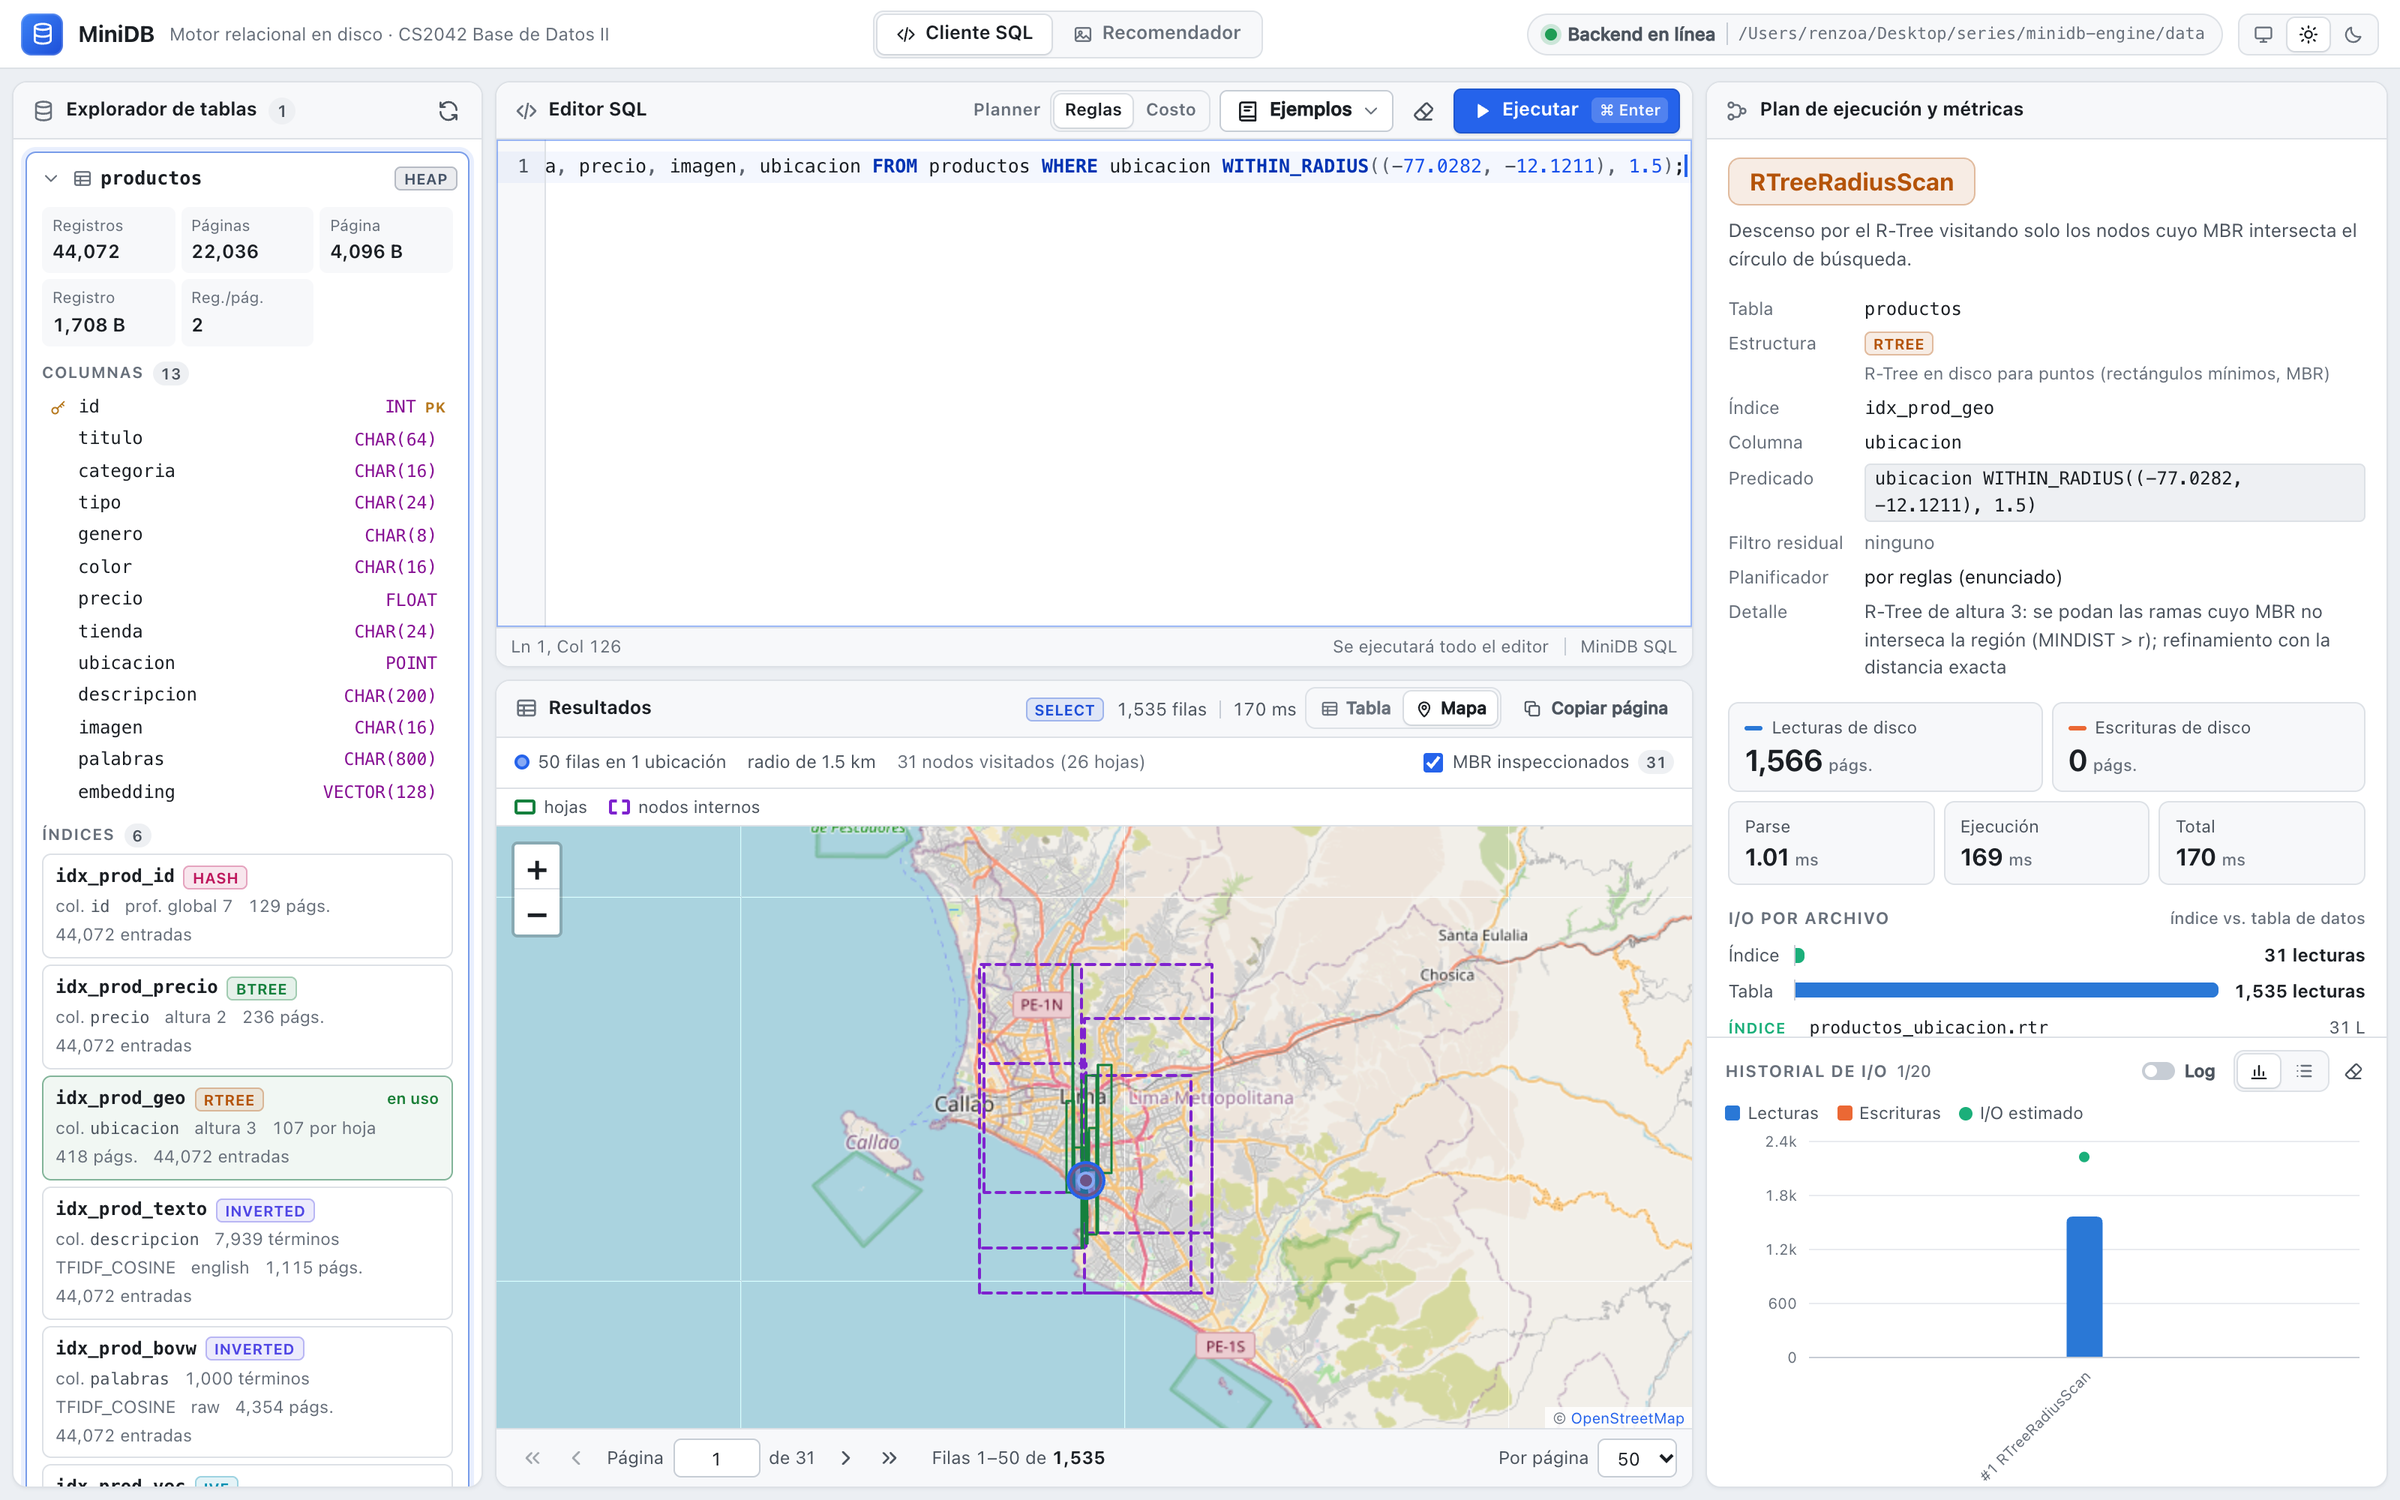
\includegraphics[width=\textwidth]{mapa.png}
\caption{Consulta \code{WITHIN\_RADIUS} en el cliente web: puntos recuperados, radio de la consulta y
cajas MBR inspeccionadas; a la derecha, el plan \code{RTreeRadiusScan} con el I/O del índice y de la
tabla.}
\label{fig:mapa}
\end{figure}

\subsection{Recomendador multimodal de moda (Opción B)}

\paragraph{Datos.} \emph{Fashion Product Images (Small)}: 44\,072 productos con imagen, nombre,
género, categoría, tipo de artículo, color, temporada y uso. El dataset no trae precio ni tienda, así
que \code{data/prepare\_fashion.py} los genera de forma determinista: un precio en soles según el
tipo de artículo y una de 140 tiendas con coordenadas en 28 distritos de Lima Metropolitana. El mismo
script extrae las imágenes, calcula los \emph{embeddings} y las palabras visuales, y con
\code{--load} crea la tabla, la carga con \code{COPY} y construye seis índices: hash sobre \code{id},
B$^+$ sobre \code{precio}, R-Tree sobre \code{ubicacion}, índice invertido sobre \code{descripcion}
(inglés), índice invertido sobre \code{palabras} (BoVW) e IVF sobre \code{embedding}.

\paragraph{Flujo.} El usuario sube la foto de una prenda (o elige un producto) y/o escribe una
descripción, y puede acotar por rango de precios y por cercanía a un punto del mapa. El backend
vectoriza la imagen con los mismos modelos del catálogo y \textbf{arma una sentencia SQL por método},
que ejecuta en el motor:

\begin{lstlisting}[style=sql]
-- Embedding + IVF
SELECT id, titulo, ..., embedding <=> '[...]' AS distancia FROM productos
WHERE precio BETWEEN 20 AND 80 AND ubicacion WITHIN_RADIUS((-77.0282, -12.1211), 6)
ORDER BY distancia ASC LIMIT 12;
-- BoVW + indice invertido
SELECT id, titulo, ..., COSINE_SCORE() AS similitud FROM productos
WHERE palabras MATCH 'v12:3 v85 v402 ...' AND precio BETWEEN 20 AND 80
  AND ubicacion WITHIN_RADIUS((-77.0282, -12.1211), 6)
ORDER BY similitud DESC LIMIT 12;
\end{lstlisting}

Como la aplicación solo usa SQL, cada método devuelve su plan y sus métricas: la interfaz muestra,
lado a lado, los productos recomendados por BoVW y por \emph{embeddings}, las lecturas de disco en el
índice y en la tabla, el tiempo, la estrategia elegida y el SQL ejecutado, y ubica las tiendas en el
mapa (figura~\ref{fig:app}). Se puede agregar el $k$-NN exacto como referencia y la búsqueda por
texto (TF-IDF sobre \code{descripcion}).

\begin{figure}[H]
\centering
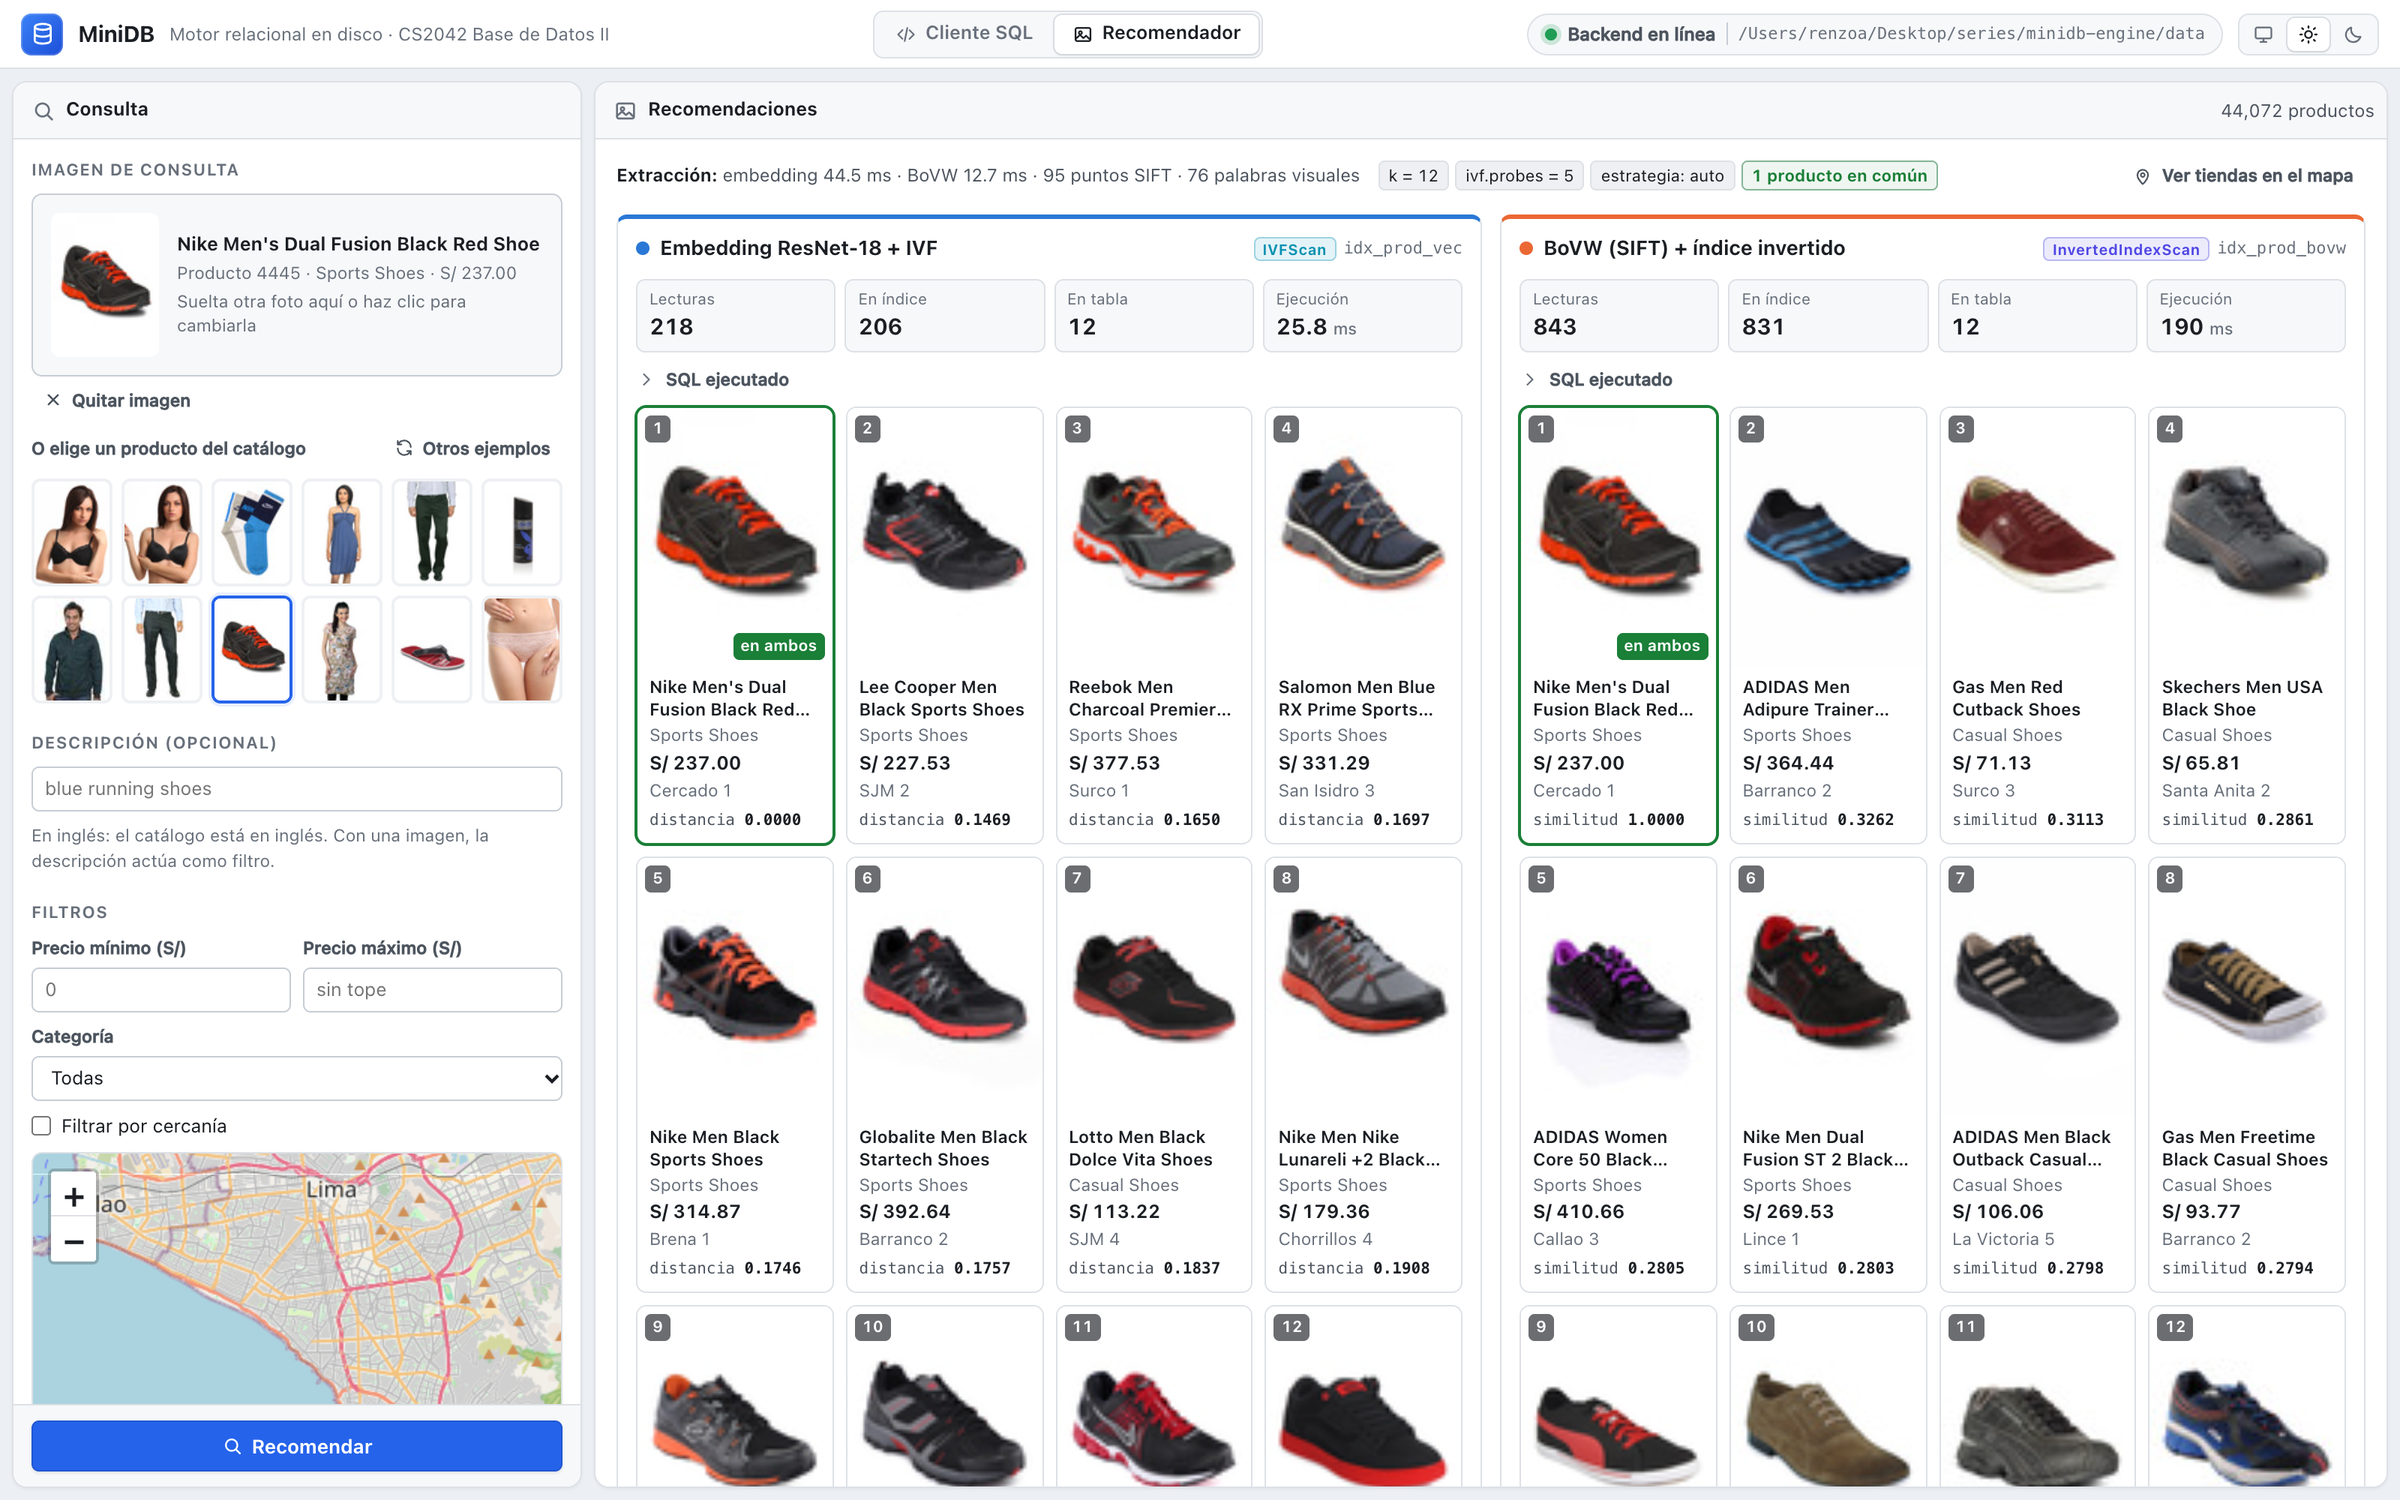
\includegraphics[width=\textwidth]{recomendador.png}
\caption{Recomendador: consulta por imagen con filtros de precio y cercanía; resultados de
\emph{Embedding + IVF} y de \emph{BoVW + índice invertido} con sus lecturas de disco.}
\label{fig:app}
\end{figure}

%==========================================================================================
\section{Experimentación}
\label{sec:experimentos}

% Sección de experimentación del Entregable 2 (se incluye desde informe_e2.tex).

\subsection{Metodología}

Los cuatro experimentos están automatizados (\code{python -m benchmarks.run\_all --only 5 6 7 8}) y
guardan CSV y PNG en \code{benchmarks/results/}. Cada uno crea archivos nuevos en una carpeta de
trabajo, con semilla fija. Salvo donde se indica, las consultas se ejecutan \textbf{por SQL sobre el
motor completo} (\code{Database.execute}), de modo que las lecturas incluyen traer los registros de
la tabla, y se toman del \code{DiskCounter} con su desglose por archivo. Entorno:
Python 3.12.13 en macOS-26.3.1-arm64-arm-64bit (10 núcleos), corrida del 2026-11-13 15:49:19%
.

Como en el Entregable~1, los bloques leídos son deterministas y son la métrica principal; los tiempos
dependen de la máquina y de la caché de páginas del sistema operativo (los archivos caben en memoria),
por lo que reflejan sobre todo el costo de CPU. El motor no tiene \emph{buffer pool}: cada lectura
informada es una transferencia real de 4\,KB.

%------------------------------------------------------------------------------------------
\subsection{Experimento 5: escalabilidad espacial y maldición de la dimensionalidad}

\paragraph{Parte A: R-Tree frente al recorrido secuencial en 2D.} Puntos (longitud, latitud) dentro
de Lima Metropolitana (70\,\% agrupados alrededor de 25 centros, 30\,\% uniformes), $N\in\{10^4,
5\cdot10^4, 10^5\}$, en una tabla \code{locales(id, nombre, ubicacion)} de 81 registros por página.
Se promedian 40 consultas por configuración con tres caminos: sin índice, con un R-Tree construido
por inserciones (el índice existe antes del \code{COPY}) y con un R-Tree empaquetado con STR
(\code{CREATE INDEX} después de cargar).

\begin{table}[H]
\centering\scriptsize
\resizebox{\ifdim\width>\textwidth\textwidth\else\width\fi}{!}{\begin{tabular}{@{}llrrrrrrr@{}}
\toprule
 & & \multicolumn{2}{c}{Secuencial (Heap)} & \multicolumn{2}{c}{R-Tree (inserciones)} & \multicolumn{2}{c}{R-Tree (STR)} & \\
\cmidrule(lr){3-4}\cmidrule(lr){5-6}\cmidrule(lr){7-8}
$N$ & consulta & lecturas & ms & lecturas & ms & lecturas & ms & filas \\
\midrule
10\,000 & radio 0.5 km & 124.0 & 13.55 & 14.8 & 0.22 & 14.8 & 0.34 & 10.2 \\
 & radio 1 km & 124.0 & 14.52 & 45.7 & 0.39 & 45.5 & 0.56 & 40.0 \\
 & radio 2 km & 124.0 & 13.54 & 151.8 & 1.14 & 150.8 & 0.95 & 143.2 \\
 & radio 5 km & 124.0 & 13.72 & 601.6 & 3.71 & 600.4 & 3.39 & 585.5 \\
 & $k$-NN, $k=5$ & 124.0 & 18.22 & 9.2 & 0.29 & 9.4 & 0.44 & 5.0 \\
 & $k$-NN, $k=20$ & 124.0 & 18.33 & 25.4 & 0.45 & 25.2 & 0.60 & 20.0 \\
 & $k$-NN, $k=50$ & 124.0 & 18.28 & 56.6 & 0.69 & 56.1 & 0.92 & 50.0 \\
\addlinespace
50\,000 & radio 0.5 km & 618.0 & 68.18 & 63.8 & 0.91 & 63.9 & 0.61 & 55.0 \\
 & radio 1 km & 618.0 & 67.78 & 222.8 & 1.82 & 221.3 & 1.66 & 208.8 \\
 & radio 2 km & 618.0 & 67.92 & 756.2 & 5.07 & 751.9 & 5.41 & 731.7 \\
 & radio 5 km & 618.0 & 71.65 & 2\,750.5 & 16.76 & 2\,736.8 & 16.98 & 2\,691.4 \\
 & $k$-NN, $k=5$ & 618.0 & 105.25 & 10.5 & 0.44 & 11.9 & 0.61 & 5.0 \\
 & $k$-NN, $k=20$ & 618.0 & 97.78 & 27.1 & 0.61 & 27.9 & 0.75 & 20.0 \\
 & $k$-NN, $k=50$ & 618.0 & 98.40 & 59.0 & 0.93 & 59.1 & 1.05 & 50.0 \\
\addlinespace
100\,000 & radio 0.5 km & 1\,235.0 & 138.98 & 104.7 & 1.15 & 102.4 & 0.83 & 92.5 \\
 & radio 1 km & 1\,235.0 & 147.25 & 375.1 & 2.56 & 369.8 & 2.81 & 354.6 \\
 & radio 2 km & 1\,235.0 & 137.20 & 1\,270.5 & 7.89 & 1\,259.8 & 8.47 & 1\,232.1 \\
 & radio 5 km & 1\,235.0 & 138.74 & 4\,568.9 & 34.00 & 4\,541.9 & 27.25 & 4\,474.6 \\
 & $k$-NN, $k=5$ & 1\,235.0 & 187.19 & 12.2 & 0.58 & 12.0 & 0.58 & 5.0 \\
 & $k$-NN, $k=20$ & 1\,235.0 & 185.63 & 28.8 & 0.72 & 28.1 & 0.77 & 20.0 \\
 & $k$-NN, $k=50$ & 1\,235.0 & 192.36 & 60.8 & 1.45 & 59.3 & 2.14 & 50.0 \\
\bottomrule
\end{tabular}
}
\caption{Experimento 5A: bloques leídos (índice + tabla) y tiempo por consulta.}
\label{tab:exp5}
\end{table}

\begin{table}[H]
\centering\small
\resizebox{\ifdim\width>\textwidth\textwidth\else\width\fi}{!}{\begin{tabular}{@{}rrrrrrrr@{}}
\toprule
$N$ & páginas del Heap & \multicolumn{3}{c}{R-Tree por inserciones} & \multicolumn{3}{c}{R-Tree STR} \\
\cmidrule(lr){3-5}\cmidrule(l){6-8}
 & & páginas & altura & construcción (s) / escrituras & páginas & altura & construcción (s) / escrituras \\
\midrule
10\,000 & 124 & 141 & 3 & 0.88 / 10\,678 & 96 & 2 & 0.02 / 100 \\
50\,000 & 618 & 696 & 3 & 5.51 / 53\,564 & 475 & 3 & 0.11 / 479 \\
100\,000 & 1\,235 & 1\,402 & 3 & 10.95 / 106\,617 & 946 & 3 & 0.21 / 950 \\
\bottomrule
\end{tabular}
}
\caption{Tamaño y costo de construcción del R-Tree. Para el árbol por inserciones se descuenta el
costo de cargar el Heap.}
\label{tab:exp5build}
\end{table}

\begin{figure}[H]
\centering
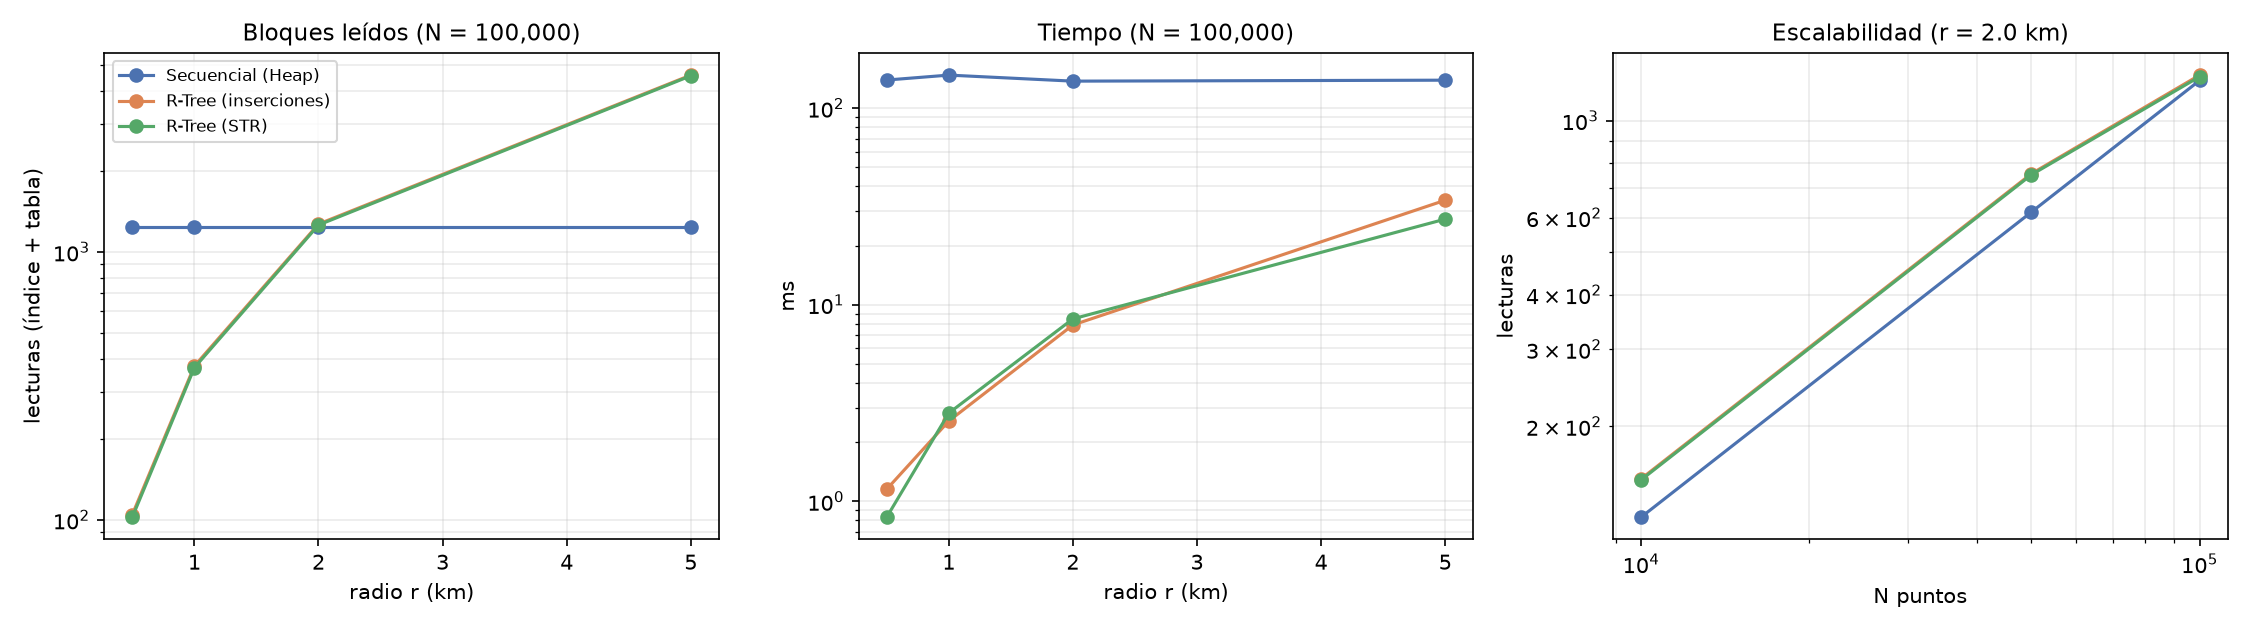
\includegraphics[width=\textwidth]{exp5_radius.png}
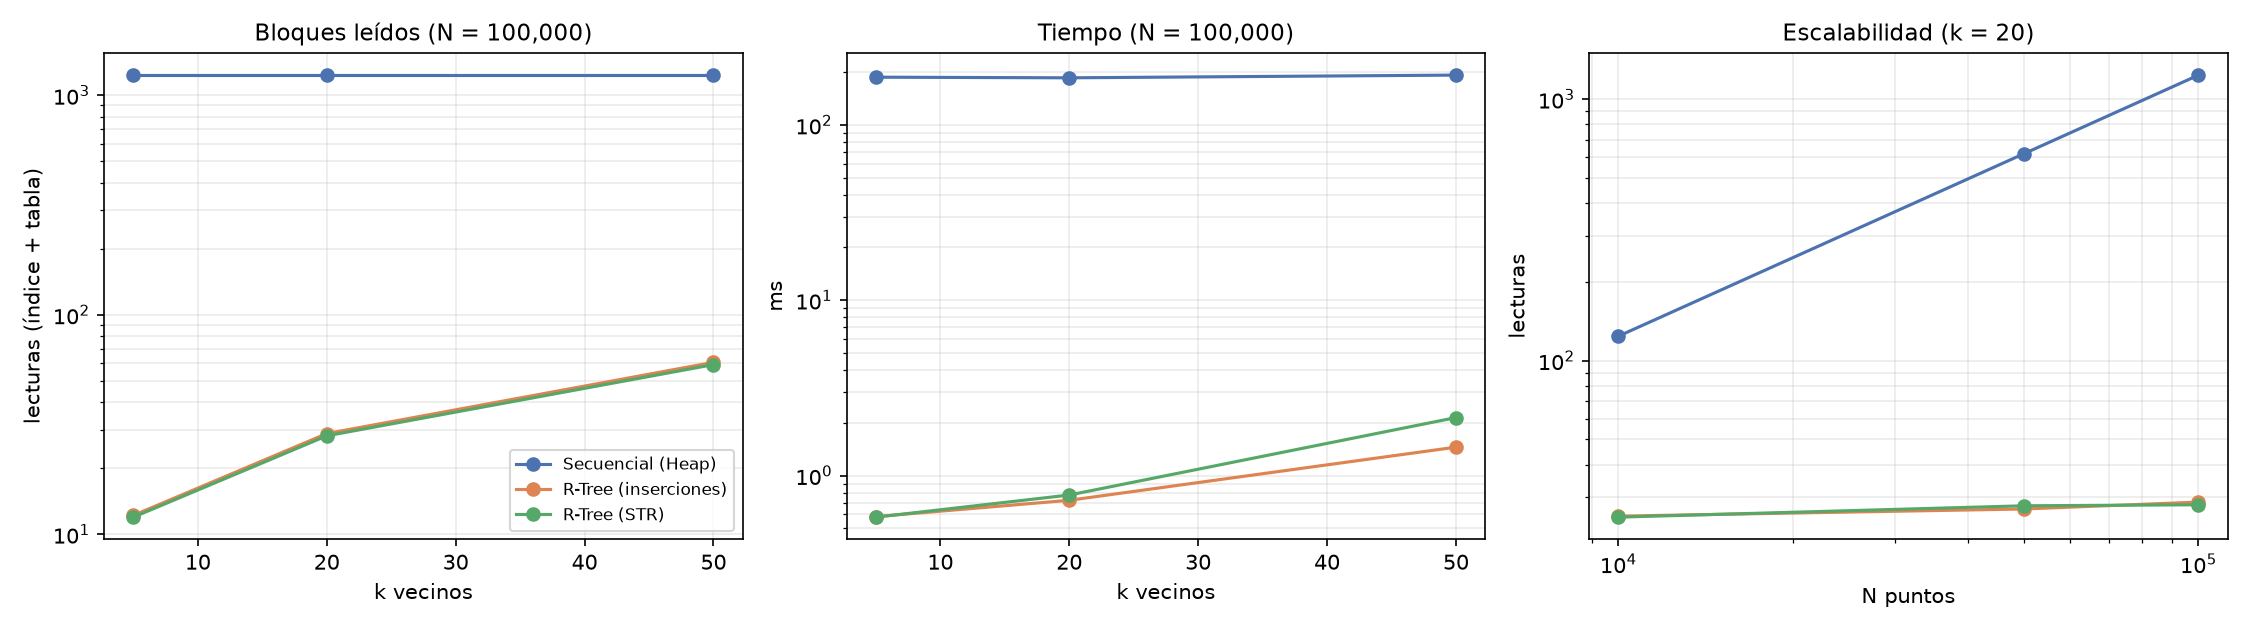
\includegraphics[width=\textwidth]{exp5_knn.png}
\caption{Experimento 5A: consultas por radio (arriba) y $k$-NN (abajo).}
\label{fig:exp5}
\end{figure}

\paragraph{Análisis.}
\begin{itemize}
\item \textbf{$k$-NN}: el R-Tree lee $h$ + unas pocas hojas + $k$ registros. Con $N=10^5$ y $k=5$
  son 12 bloques (7 del índice y 5 de la tabla) frente a los 1\,235 del recorrido secuencial, y el
  costo casi no crece con $N$ (9, 11 y 12 lecturas para $10^4$, $5\cdot10^4$ y $10^5$): solo depende
  de la altura. El recorrido secuencial crece linealmente con $N$.
\item \textbf{Radio}: el índice visita pocos nodos (10 a 94) pero, como no está agrupado, paga una
  lectura de la tabla por cada punto que califica. Con radios pequeños gana por un orden de magnitud
  (102 frente a 1\,235 bloques con $r=0.5$\,km); cuando califican más filas que páginas tiene la
  tabla ($r\ge2$\,km con $N=10^5$) lee \emph{más} bloques que el recorrido secuencial, el mismo
  cruce que observamos con el B$^+$ no agrupado en el Experimento~3. En tiempo sigue ganando (8\,ms
  frente a 137\,ms con $r=2$\,km) porque el recorrido secuencial decodifica y evalúa las $10^5$ filas.
\item \textbf{Inserciones frente a STR}: el árbol empaquetado ocupa un 33\,\% menos de páginas (hojas
  llenas en lugar de $\approx$70\,\%) y se construye con una escritura por página: 950 escrituras
  frente a 106\,617 (cada inserción cuesta $h$ lecturas y al menos una escritura). En consultas ambos
  leen prácticamente lo mismo; el STR visita algo menos de nodos en los radios grandes (67 frente a 94
  con $r=5$\,km) porque sus cajas se solapan menos.
\end{itemize}

\paragraph{Parte B: efecto de la dimensión.} $N=20\,000$ vectores uniformes en $[0,1]^D$ con
coordenadas \code{float32}; $k$-NN con $k=10$ (30 consultas) sobre un R-Tree construido por
inserciones, frente al recorrido secuencial de un Heap con los mismos vectores (ambos con $B=4096$).

\begin{table}[H]
\centering\small
\begin{tabular}{@{}lrrrrrrr@{}}
\toprule
Dimensión $D$ & 2 & 4 & 8 & 16 & 32 & 64 & 128 \\
\midrule
entradas por hoja & 185 & 107 & 58 & 30 & 15 & 7 & 3 \\
altura del R-Tree & 2 & 3 & 3 & 4 & 4 & 6 & 11 \\
páginas del R-Tree & 159 & 279 & 508 & 955 & 1\,745 & 3\,797 & 11\,092 \\
páginas del Heap ($P$) & 60 & 100 & 179 & 339 & 667 & 1\,334 & 2\,858 \\
R-Tree: lecturas por $k$-NN & 12.7 & 21.5 & 100.3 & 952.5 & 1\,754.0 & 3\,806.0 & 11\,100.9 \\
R-Tree: \% de hojas visitadas & 1.1 & 3.2 & 16.4 & 98.7 & 100.0 & 100.0 & 100.0 \\
Secuencial: lecturas & 60 & 100 & 179 & 339 & 667 & 1\,334 & 2\,858 \\
R-Tree: ms por consulta & 0.32 & 1.12 & 4.70 & 42.72 & 51.17 & 79.92 & 190.49 \\
Secuencial: ms por consulta & 7.72 & 11.78 & 9.37 & 13.76 & 12.14 & 18.33 & 31.38 \\
\bottomrule
\end{tabular}

\caption{Experimento 5B: $k$-NN ($k=10$) según la dimensión.}
\label{tab:exp5dim}
\end{table}

\begin{figure}[H]
\centering
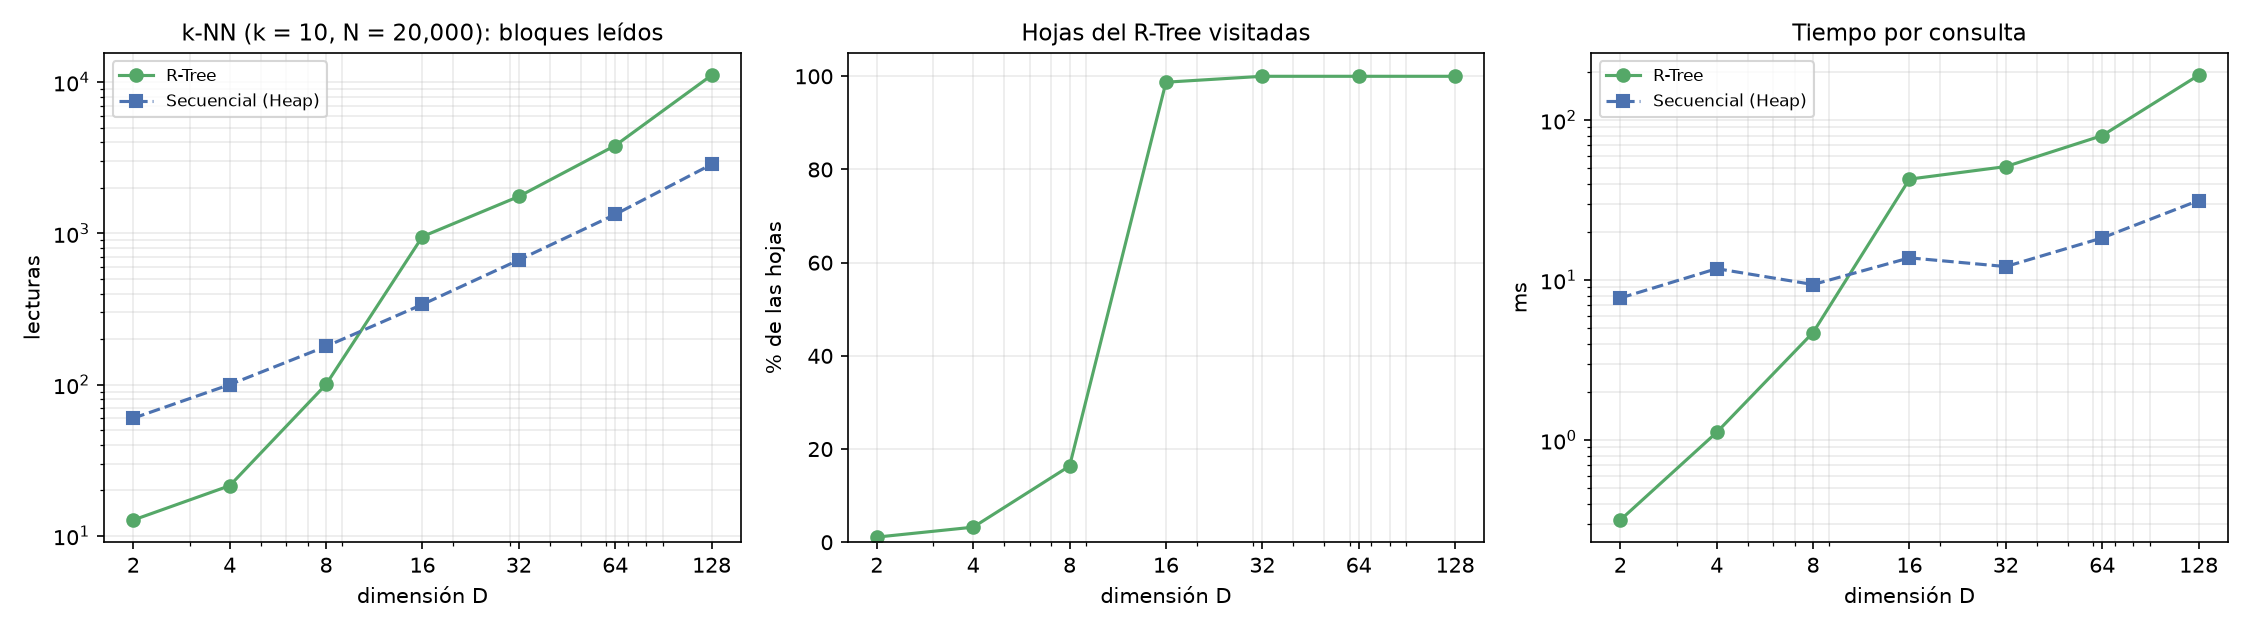
\includegraphics[width=\textwidth]{exp5_dimension.png}
\caption{Experimento 5B: bloques leídos, fracción de hojas visitadas y tiempo según $D$.}
\label{fig:exp5dim}
\end{figure}

\paragraph{Análisis.} El R-Tree gana con claridad en $D=2$ y $D=4$ (13 y 21 lecturas frente a 60 y
100) y todavía en $D=8$ (100 frente a 179), pero \textbf{desde $D=16$ pierde}: visita el 99\,\% de
las hojas y lee 953 bloques frente a los 339 del recorrido secuencial. Actúan dos efectos a la vez.
Primero, la entrada crece como $2Dc$ y el \emph{fan-out} cae de 185 a 3 entradas por página, así que
el árbol tiene más páginas que la propia tabla (11\,092 frente a 2\,858 con $D=128$) y su altura
pasa de 2 a 11. Segundo, en alta dimensión las distancias se concentran: la distancia al vecino más
cercano se parece a la del más lejano, las cajas se solapan y $\text{MINDIST}$ deja de podar, por lo
que el recorrido \emph{best-first} termina abriendo todos los nodos. Es la maldición de la
dimensionalidad: para los vectores de 128 dimensiones de la aplicación un índice espacial exacto no
sirve, y por eso el módulo vectorial usa un índice aproximado (Experimento~8).

%------------------------------------------------------------------------------------------
\subsection{Experimento 6: índice invertido frente a \emph{full scan} y GIN de PostgreSQL}

Corpus: las descripciones de los productos (en inglés, 12.7 términos por documento tras el
preprocesamiento), de 1\,000 a 44\,072 documentos en una tabla \code{docs(id, cuerpo TEXT(200))} de
19 registros por página. PostgreSQL~18 con \code{GIN (to\_tsvector('english', cuerpo))}.

\begin{table}[H]
\centering\small
\resizebox{\ifdim\width>\textwidth\textwidth\else\width\fi}{!}{\begin{tabular}{@{}rrrrrrrrrr@{}}
\toprule
 & \multicolumn{7}{c}{MiniDB: índice invertido en disco} & \multicolumn{2}{c}{PostgreSQL GIN} \\
\cmidrule(lr){2-8}\cmidrule(l){9-10}
documentos & términos & posteos & vocab. & posteos & docs & total (KB) & s & KB & s \\
\midrule
1\,000 & 1\,010 & 12\,722 & 15 & 19 & 4 & 164 & 0.03 & 104 & 0.03 \\
2\,000 & 1\,492 & 25\,377 & 21 & 38 & 8 & 280 & 0.06 & 160 & 0.04 \\
5\,000 & 2\,398 & 63\,538 & 34 & 94 & 20 & 604 & 0.12 & 296 & 0.10 \\
10\,000 & 3\,676 & 127\,061 & 52 & 188 & 40 & 1\,132 & 0.21 & 544 & 0.18 \\
20\,000 & 5\,455 & 254\,178 & 76 & 375 & 80 & 2\,136 & 0.39 & 968 & 0.36 \\
44\,072 & 7\,939 & 560\,112 & 111 & 827 & 174 & 4\,460 & 0.92 & 1\,824 & 0.73 \\
\bottomrule
\end{tabular}
}
\caption{Experimento 6: construcción del índice. Para MiniDB se indican las páginas de cada archivo
(\code{vocab.dic}, \code{postings.inv}, \code{docs.bin}), el tamaño total y el tiempo.}
\label{tab:exp6build}
\end{table}

\begin{figure}[H]
\centering
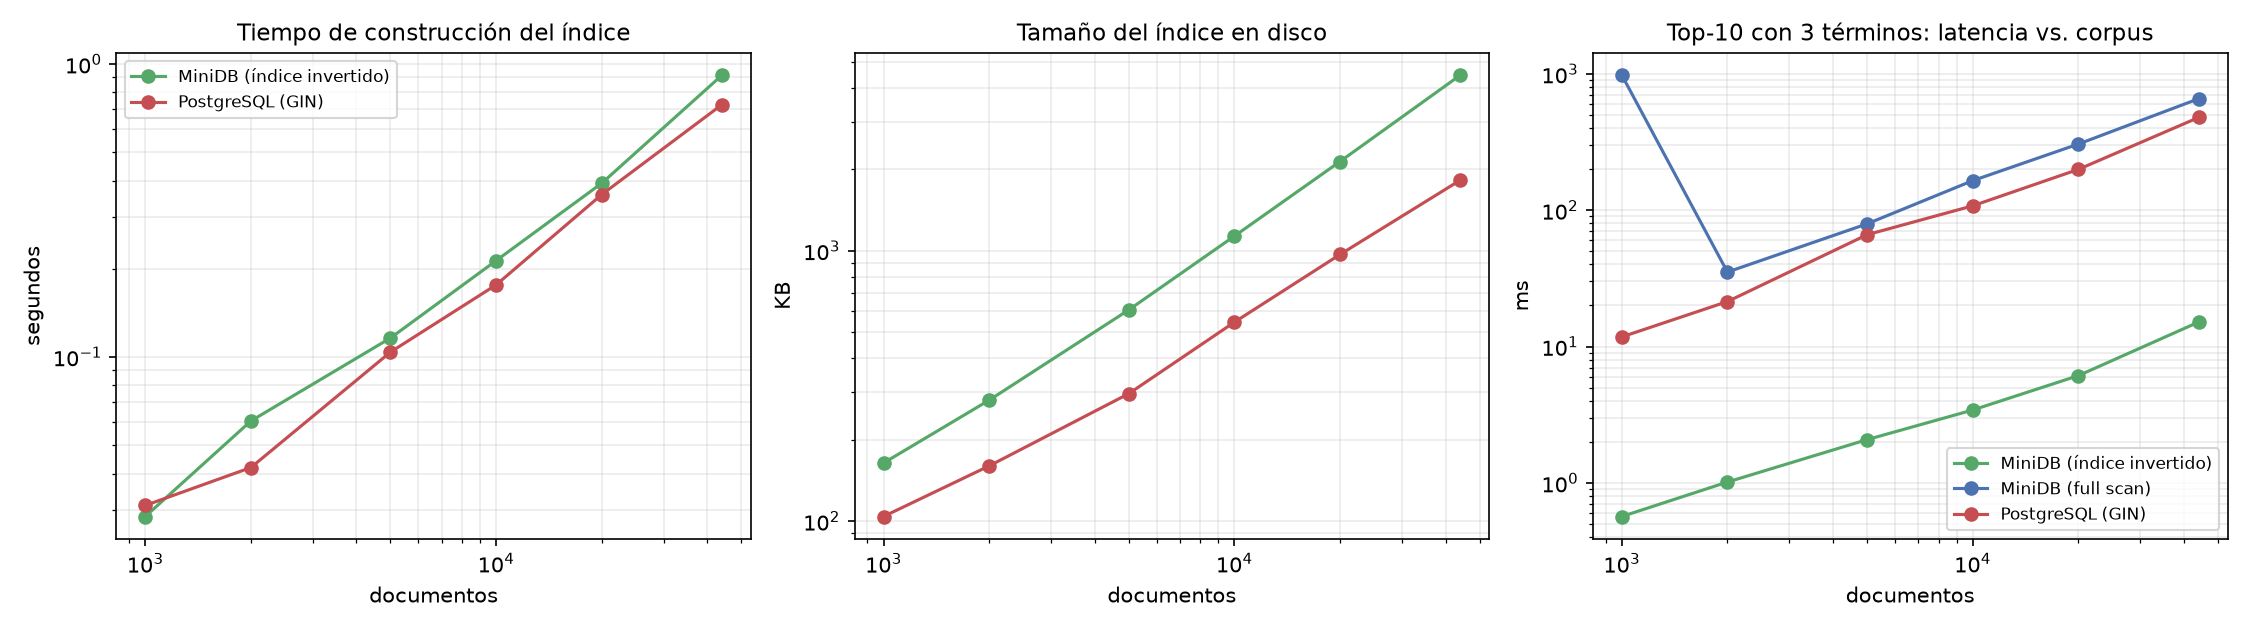
\includegraphics[width=\textwidth]{exp6_build.png}
\caption{Experimento 6: tiempo de construcción, tamaño en disco y latencia del Top-10 de 3 términos
según el tamaño del corpus.}
\label{fig:exp6build}
\end{figure}

\paragraph{Construcción.} El tiempo y el tamaño crecen linealmente con el corpus: el vocabulario
crece de forma sublineal (ley de Heaps: 1\,010 términos con 1\,000 documentos y 7\,939 con 44\,072)
y los posteos de forma lineal (12.7 por documento, 6 bytes cada uno). El índice completo de 44\,072
documentos ocupa 4.5\,MB y se construye en 0.9\,s con 3\,166 lecturas (el recorrido de la tabla y la
relectura del \emph{run}) y 1\,966 escrituras. El GIN de PostgreSQL es 2.4 veces más compacto porque
comprime las listas de posteo y no guarda frecuencias ni normas (por eso su ranking debe recalcular
el \code{tsvector} de cada documento); su tiempo de construcción es similar.

Con el corpus completo se ejecutan 30 consultas por configuración, con términos tomados de un mismo
documento para que tengan resultados (3 consultas en el caso del \emph{full scan}).

\begin{table}[H]
\centering\scriptsize
\resizebox{\ifdim\width>\textwidth\textwidth\else\width\fi}{!}{\begin{tabular}{@{}lrrrrrrrr@{}}
\toprule
 & & \multicolumn{2}{c}{MiniDB (índice invertido)} & \multicolumn{2}{c}{MiniDB (full scan)} & \multicolumn{2}{c}{PostgreSQL (GIN)} & \\
\cmidrule(lr){3-4}\cmidrule(lr){5-6}\cmidrule(lr){7-8}
consulta & términos & ms & bloques & ms & bloques & ms & bloques & filas \\
\midrule
AND & 1 & 70.20 & 13\,577.4 & 608.17 & 2\,320.0 & 2.02 & 681.9 & 13\,470.8 \\
 & 3 & 11.21 & 1\,072.8 & 589.85 & 2\,320.0 & 0.58 & 250.4 & 939.5 \\
 & 5 & 8.62 & 393.8 & 594.63 & 2\,320.0 & 0.52 & 142.7 & 213.9 \\
\addlinespace
OR & 1 & 55.07 & 10\,284.4 & 557.42 & 2\,320.0 & 1.55 & 610.6 & 10\,183.2 \\
 & 3 & 163.23 & 31\,055.6 & 609.24 & 2\,320.0 & 5.12 & 826.1 & 30\,885.4 \\
 & 5 & 215.37 & 39\,937.5 & 614.83 & 2\,320.0 & 7.99 & 837.3 & 39\,703.4 \\
\addlinespace
AND NOT & 1 & 58.15 & 10\,802.3 & 589.86 & 2\,320.0 & 2.30 & 561.1 & 10\,672.6 \\
 & 3 & 11.11 & 1\,246.8 & 594.24 & 2\,320.0 & 0.83 & 282.0 & 1\,084.8 \\
 & 5 & 11.69 & 873.4 & 602.59 & 2\,320.0 & 0.98 & 260.4 & 645.8 \\
\addlinespace
Top-10 & 1 & 5.58 & 128.1 & 625.34 & 2\,320.0 & 201.23 & 678.2 & 10.0 \\
 & 3 & 15.12 & 200.7 & 656.90 & 2\,320.0 & 478.80 & 821.8 & 10.0 \\
 & 5 & 20.76 & 251.8 & 690.45 & 2\,320.0 & 591.06 & 838.5 & 10.0 \\
\bottomrule
\end{tabular}
}
\caption{Experimento 6: latencia y bloques leídos por consulta ($N=44\,072$). MiniDB usa bloques de
4\,KB sin caché; PostgreSQL, \emph{buffers} de 8\,KB. La última columna son las filas que califican
(10 en el Top-10).}
\label{tab:exp6}
\end{table}

\begin{table}[H]
\centering\small
\begin{tabular}{@{}lrrrr@{}}
\toprule
consulta & términos & lecturas en el índice & lecturas en la tabla & filas \\
\midrule
AND & 1 & 106.6 & 13\,470.8 & 13\,470.8 \\
 & 3 & 133.3 & 939.5 & 939.5 \\
 & 5 & 179.9 & 213.9 & 213.9 \\
OR & 1 & 101.2 & 10\,183.2 & 10\,183.2 \\
 & 3 & 170.2 & 30\,885.4 & 30\,885.4 \\
 & 5 & 234.1 & 39\,703.4 & 39\,703.4 \\
AND NOT & 1 & 129.7 & 10\,672.6 & 10\,672.6 \\
 & 3 & 162.0 & 1\,084.8 & 1\,084.8 \\
 & 5 & 227.6 & 645.8 & 645.8 \\
Top-10 & 1 & 118.1 & 10.0 & 10.0 \\
 & 3 & 190.7 & 10.0 & 10.0 \\
 & 5 & 241.8 & 10.0 & 10.0 \\
\bottomrule
\end{tabular}

\caption{Desglose de las lecturas del índice invertido de MiniDB: en el índice (diccionario, posteos
y normas) y en la tabla (un registro por fila devuelta).}
\label{tab:exp6io}
\end{table}

\begin{figure}[H]
\centering
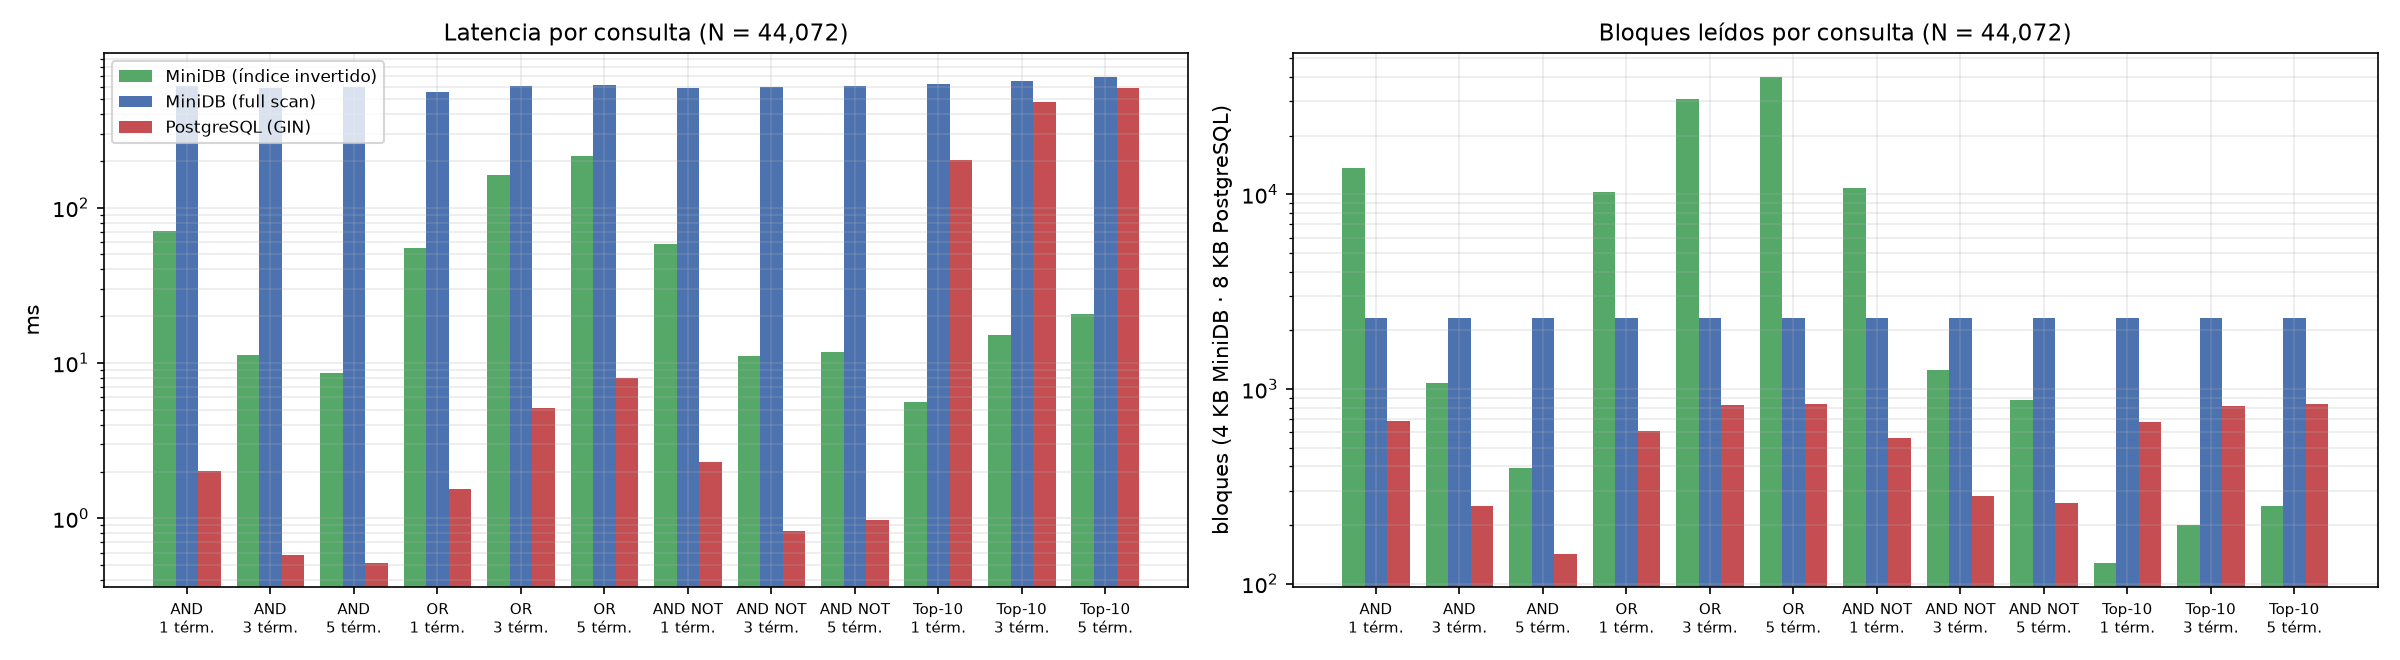
\includegraphics[width=\textwidth]{exp6_queries.png}
\caption{Experimento 6: latencia y bloques leídos por tipo de consulta y número de términos.}
\label{fig:exp6}
\end{figure}

\paragraph{Análisis.}
\begin{itemize}
\item \textbf{Correctitud}: las consultas booleanas devuelven las mismas filas en MiniDB y en
  PostgreSQL (13\,470.8 frente a 13\,469.7 en promedio para un término; las diferencias mínimas
  vienen de las listas de \emph{stopwords}), lo que valida el preprocesamiento y las mezclas con dos
  punteros.
\item \textbf{Índice frente a \emph{full scan}}: el recorrido secuencial lee siempre las 2\,320
  páginas y tokeniza los 44\,072 documentos ($\approx$600\,ms). El índice lee entre 101 y 234 bloques
  propios: $T\lceil\log_2 111\rceil$ del diccionario más las páginas de posteo de cada término. Para
  el Top-10 el total es de 128 a 252 bloques (9 a 18 veces menos que el \emph{full scan}) y la
  latencia de 6 a 21\,ms (30 a 110 veces menos).
\item \textbf{El costo está en traer las filas}: en las consultas booleanas poco selectivas
  (un término, u \code{OR} de varios) califican decenas de miles de documentos y, como el índice
  devuelve RID de un Heap no agrupado, se paga una lectura por fila: 39\,703 lecturas para un
  \code{OR} de 5 términos, más que las 2\,320 del \emph{full scan}. Es el mismo cruce de los índices
  no agrupados. Con \code{AND} de 3 o 5 términos (cientos de filas) el índice vuelve a ganar, y el
  ranking Top-$K$ evita el problema porque solo trae $K$ registros.
\item \textbf{Frente a GIN}: en consultas booleanas PostgreSQL es de 15 a 35 veces más rápido (está
  escrito en C, usa \emph{buffer pool} y un \emph{bitmap heap scan} que lee cada página de la tabla
  una sola vez, con $\approx$50 filas por página de 8\,KB). En el \textbf{ranking Top-10 MiniDB es de
  28 a 36 veces más rápido} (5.6 a 20.8\,ms frente a 201 a 591\,ms): GIN no guarda frecuencias ni
  normas, así que \code{ts\_rank} tiene que recalcular el \code{tsvector} de \emph{todos} los
  documentos que califican antes de ordenar, mientras que nuestro índice tiene $tf$ en los posteos y
  la norma precalculada en \code{docs.bin}, y solo trae de la tabla los 10 ganadores.
\item \textbf{Escalabilidad} (figura~\ref{fig:exp6build}, derecha): la latencia del Top-10 crece
  linealmente con el corpus en los tres sistemas, pero con pendientes muy distintas, porque el índice
  solo recorre las listas de los términos de la consulta.
\end{itemize}

%------------------------------------------------------------------------------------------
\subsection{Experimento 7: BoVW frente a \emph{embeddings} densos}

300 imágenes de consulta: 20 de cada uno de los 15 tipos de artículo más frecuentes. Para cada una
se recuperan sus 10 vecinos (excluida la propia imagen) por SQL sobre la tabla \code{productos}; un
resultado es relevante si es del mismo tipo de artículo.

\begin{table}[H]
\centering\small
\resizebox{\ifdim\width>\textwidth\textwidth\else\width\fi}{!}{\begin{tabular}{@{}lrrrrrrr@{}}
\toprule
Representación & P@5 & P@10 & extracción (ms/imagen) & consulta (ms) & lecturas & en el índice & índice (MB) \\
\midrule
BoVW (SIFT + índice invertido) & 0.531 & 0.505 & 7.70 & 133.68 & 646.0 & 635.0 & 17.0 \\
Embedding (ResNet-18 + IVF) & 0.811 & 0.789 & 7.80 & 6.11 & 215.6 & 204.6 & 25.1 \\
Embedding (k-NN exacto) & 0.811 & 0.786 & 7.80 & 850.25 & 22\,036.0 & 0.0 & -- \\
\bottomrule
\end{tabular}
}
\caption{Experimento 7: precisión, tiempo de extracción por imagen (medido una a una, como en una
consulta de la aplicación) y costo de la consulta.}
\label{tab:exp7}
\end{table}

\begin{figure}[H]
\centering
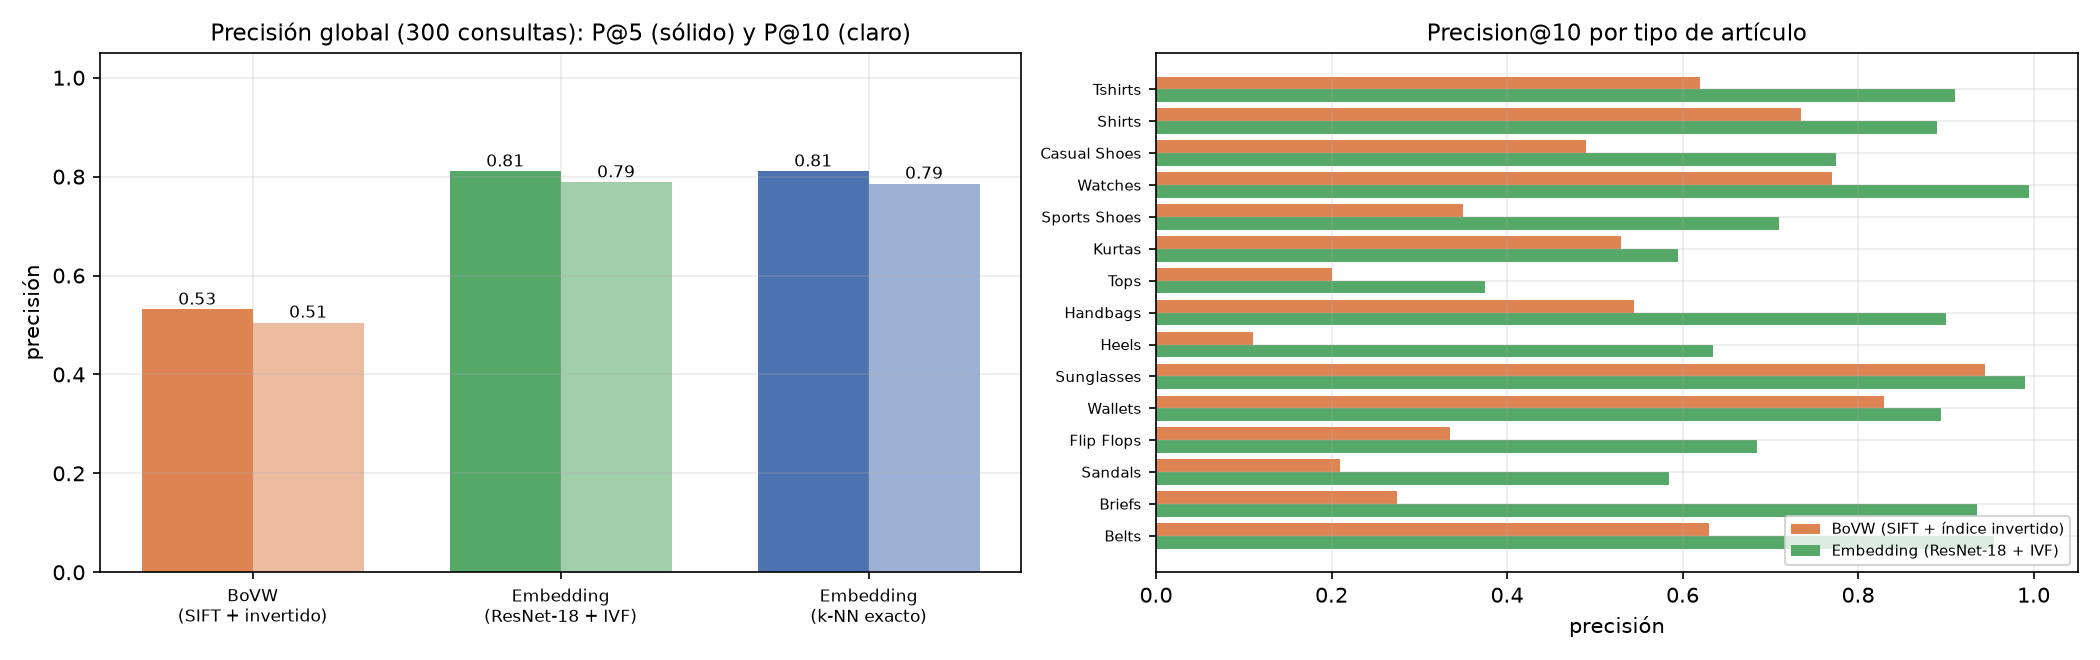
\includegraphics[width=\textwidth]{exp7_precision.png}
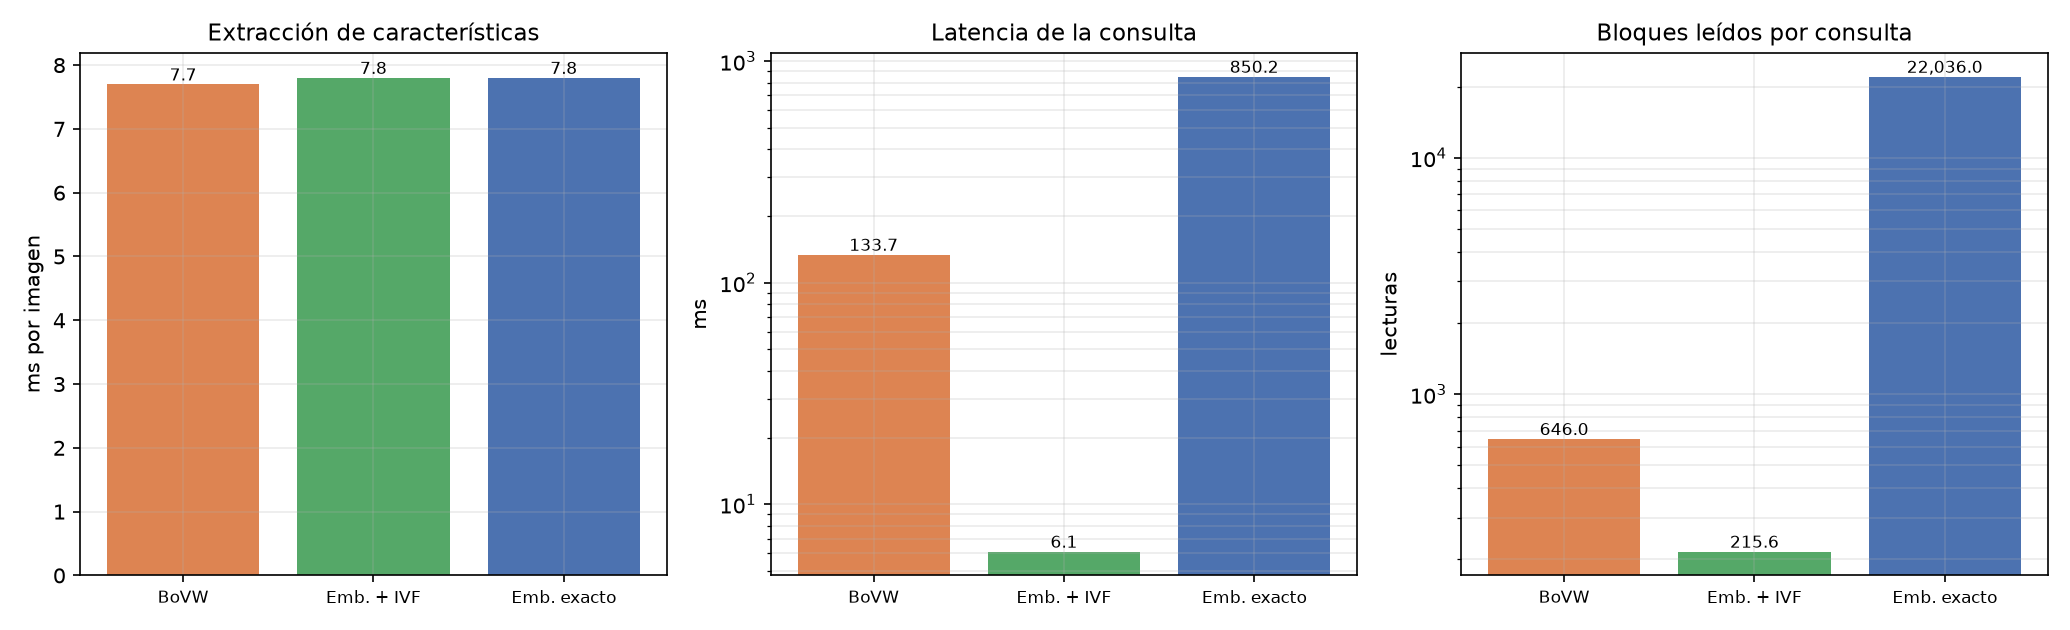
\includegraphics[width=0.92\textwidth]{exp7_cost.png}
\caption{Experimento 7: precisión global y por tipo de artículo (arriba) y costos (abajo).}
\label{fig:exp7}
\end{figure}

\begin{table}[H]
\centering\scriptsize
\resizebox{\ifdim\width>\textwidth\textwidth\else\width\fi}{!}{\begin{tabular}{@{}lrrrrrr@{}}
\toprule
 & \multicolumn{2}{c}{BoVW} & \multicolumn{2}{c}{Embedding + IVF} & \multicolumn{2}{c}{Embedding exacto} \\
Tipo de artículo & P@5 & P@10 & P@5 & P@10 & P@5 & P@10 \\
\midrule
Tshirts & 0.63 & 0.62 & 0.93 & 0.91 & 0.93 & 0.91 \\
Shirts & 0.82 & 0.73 & 0.91 & 0.89 & 0.92 & 0.90 \\
Casual Shoes & 0.52 & 0.49 & 0.81 & 0.78 & 0.82 & 0.79 \\
Watches & 0.76 & 0.77 & 1.00 & 0.99 & 1.00 & 0.99 \\
Sports Shoes & 0.34 & 0.35 & 0.71 & 0.71 & 0.73 & 0.71 \\
Kurtas & 0.61 & 0.53 & 0.62 & 0.59 & 0.64 & 0.60 \\
Tops & 0.30 & 0.20 & 0.47 & 0.38 & 0.46 & 0.36 \\
Handbags & 0.56 & 0.55 & 0.89 & 0.90 & 0.89 & 0.90 \\
Heels & 0.10 & 0.11 & 0.68 & 0.64 & 0.66 & 0.60 \\
Sunglasses & 0.95 & 0.94 & 0.98 & 0.99 & 0.98 & 0.99 \\
Wallets & 0.87 & 0.83 & 0.92 & 0.90 & 0.92 & 0.90 \\
Flip Flops & 0.37 & 0.34 & 0.71 & 0.69 & 0.69 & 0.68 \\
Sandals & 0.20 & 0.21 & 0.63 & 0.58 & 0.62 & 0.58 \\
Briefs & 0.29 & 0.28 & 0.95 & 0.94 & 0.95 & 0.94 \\
Belts & 0.65 & 0.63 & 0.95 & 0.95 & 0.95 & 0.95 \\
\bottomrule
\end{tabular}
}
\caption{Experimento 7: precisión por tipo de artículo.}
\label{tab:exp7tipos}
\end{table}

\paragraph{Análisis.}
\begin{itemize}
\item \textbf{Efectividad}: los \emph{embeddings} alcanzan P@10 = 0.79 frente a 0.51 del BoVW, y
  ganan en los 15 tipos. El BoVW funciona bien cuando la categoría tiene una textura local
  característica (gafas 0.95, billeteras 0.83, relojes 0.77, camisas 0.74) y falla cuando lo que
  distingue a la prenda es la forma global o es parecida a otra categoría: tacones (0.11), sandalias
  (0.21), \emph{tops} (0.20). SIFT describe esquinas y bordes locales, y el histograma descarta la
  disposición espacial; además, en imágenes de $60\times80$ hay pocos puntos de interés (75 en
  promedio). La ResNet-18 codifica forma y contexto global aprendidos en ImageNet. Las dos
  representaciones confunden categorías visualmente cercanas (\emph{tops} con camisetas, sandalias
  con chanclas).
\item \textbf{IVF frente a exacto}: la precisión del índice aproximado con \code{probes} = 5 es
  indistinguible de la del $k$-NN exacto (0.789 y 0.786): los pocos vecinos que el IVF cambia son
  igual de relevantes.
\item \textbf{Extracción}: ambas cuestan $\approx$8\,ms por imagen (SIFT en CPU; ResNet-18 en la GPU
  integrada, 4.2\,ms por imagen en lotes de 256). El BoVW necesita además entrenar el \emph{codebook}
  (37\,s de K-Means para 1\,000 palabras).
\item \textbf{Consulta}: el \emph{embedding} con IVF responde en 6\,ms leyendo 216 bloques; el BoVW
  tarda 134\,ms y lee 646, porque una imagen de consulta tiene $\approx$64 palabras visuales, muchas
  muy frecuentes (un vocabulario de solo 1\,000 palabras repartido en 44\,072 imágenes da listas de
  posteo de miles de entradas), y hay que recorrer la lista de cada una. El $k$-NN exacto lee las
  22\,036 páginas de la tabla (850\,ms).
\end{itemize}

%------------------------------------------------------------------------------------------
\subsection{Experimento 8: eficiencia frente a calidad en la búsqueda aproximada}

200 consultas (vectores del catálogo con ruido gaussiano, renormalizados) sobre los 44\,072
\emph{embeddings} de 128 dimensiones; $k=10$. La verdad base es el $k$-NN lineal exacto. Se varía
\code{ivf.probes} y el número de celdas (\code{lists} $=\sqrt N/4$, $\sqrt N$ y $4\sqrt N$).

\begin{table}[H]
\centering\scriptsize
\resizebox{\ifdim\width>\textwidth\textwidth\else\width\fi}{!}{\begin{tabular}{@{}rrrrrrrr@{}}
\toprule
\code{lists} & \code{probes} & Recall@10 (\%) & ms & lecturas & en el índice & en la tabla & vectores comparados (\%) \\
\midrule
52 & 1 & 80.8 & 2.68 & 161.3 & 151.3 & 10.0 & 2.3 \\
 & 2 & 92.7 & 4.77 & 293.6 & 283.6 & 10.0 & 4.4 \\
 & 5 & 99.2 & 11.32 & 676.3 & 666.3 & 10.0 & 10.4 \\
 & 10 & 99.9 & 21.77 & 1\,296.7 & 1\,286.7 & 10.0 & 20.2 \\
 & 20 & 99.9 & 42.79 & 2\,433.3 & 2\,423.3 & 10.0 & 38.2 \\
 & 50 & 99.9 & 111.70 & 6\,070.5 & 6\,060.5 & 10.0 & 95.8 \\
 & 52 & 100.0 & 112.79 & 6\,336.0 & 6\,326.0 & 10.0 & 100.0 \\
\addlinespace
209 & 1 & 69.4 & 1.08 & 76.5 & 66.5 & 10.0 & 0.6 \\
 & 2 & 84.1 & 1.97 & 112.1 & 102.1 & 10.0 & 1.1 \\
 & 5 & 95.9 & 3.23 & 211.8 & 201.8 & 10.0 & 2.7 \\
 & 10 & 98.6 & 5.79 & 363.0 & 353.0 & 10.0 & 5.1 \\
 & 20 & 99.5 & 11.12 & 667.7 & 657.7 & 10.0 & 9.8 \\
 & 50 & 99.9 & 27.25 & 1\,556.9 & 1\,546.9 & 10.0 & 23.8 \\
 & 100 & 100.0 & 51.47 & 3\,030.7 & 3\,020.7 & 10.0 & 46.8 \\
 & 209 & 99.9 & 111.22 & 6\,425.0 & 6\,415.0 & 10.0 & 100.0 \\
\addlinespace
836 & 1 & 57.7 & 1.30 & 140.7 & 130.7 & 10.0 & 0.2 \\
 & 2 & 73.2 & 1.41 & 151.2 & 141.2 & 10.0 & 0.3 \\
 & 5 & 88.9 & 1.98 & 180.9 & 170.9 & 10.0 & 0.8 \\
 & 10 & 95.5 & 2.85 & 228.8 & 218.8 & 10.0 & 1.5 \\
 & 20 & 98.6 & 4.11 & 315.3 & 305.3 & 10.0 & 2.8 \\
 & 50 & 99.8 & 8.33 & 559.1 & 549.1 & 10.0 & 6.5 \\
 & 100 & 100.0 & 15.16 & 955.4 & 945.4 & 10.0 & 12.4 \\
 & 836 & 99.9 & 116.99 & 6\,786.0 & 6\,776.0 & 10.0 & 100.0 \\
\addlinespace
\multicolumn{2}{@{}l}{$k$-NN exacto (secuencial)} & 100.0 & 878.85 & 22\,036.0 & 0.0 & 22\,036.0 & 100.0 \\
\bottomrule
\end{tabular}
}
\caption{Experimento 8: Recall@10, latencia y bloques leídos (directorio y listas del IVF, más los 10
registros de la tabla).}
\label{tab:exp8}
\end{table}

\begin{figure}[H]
\centering
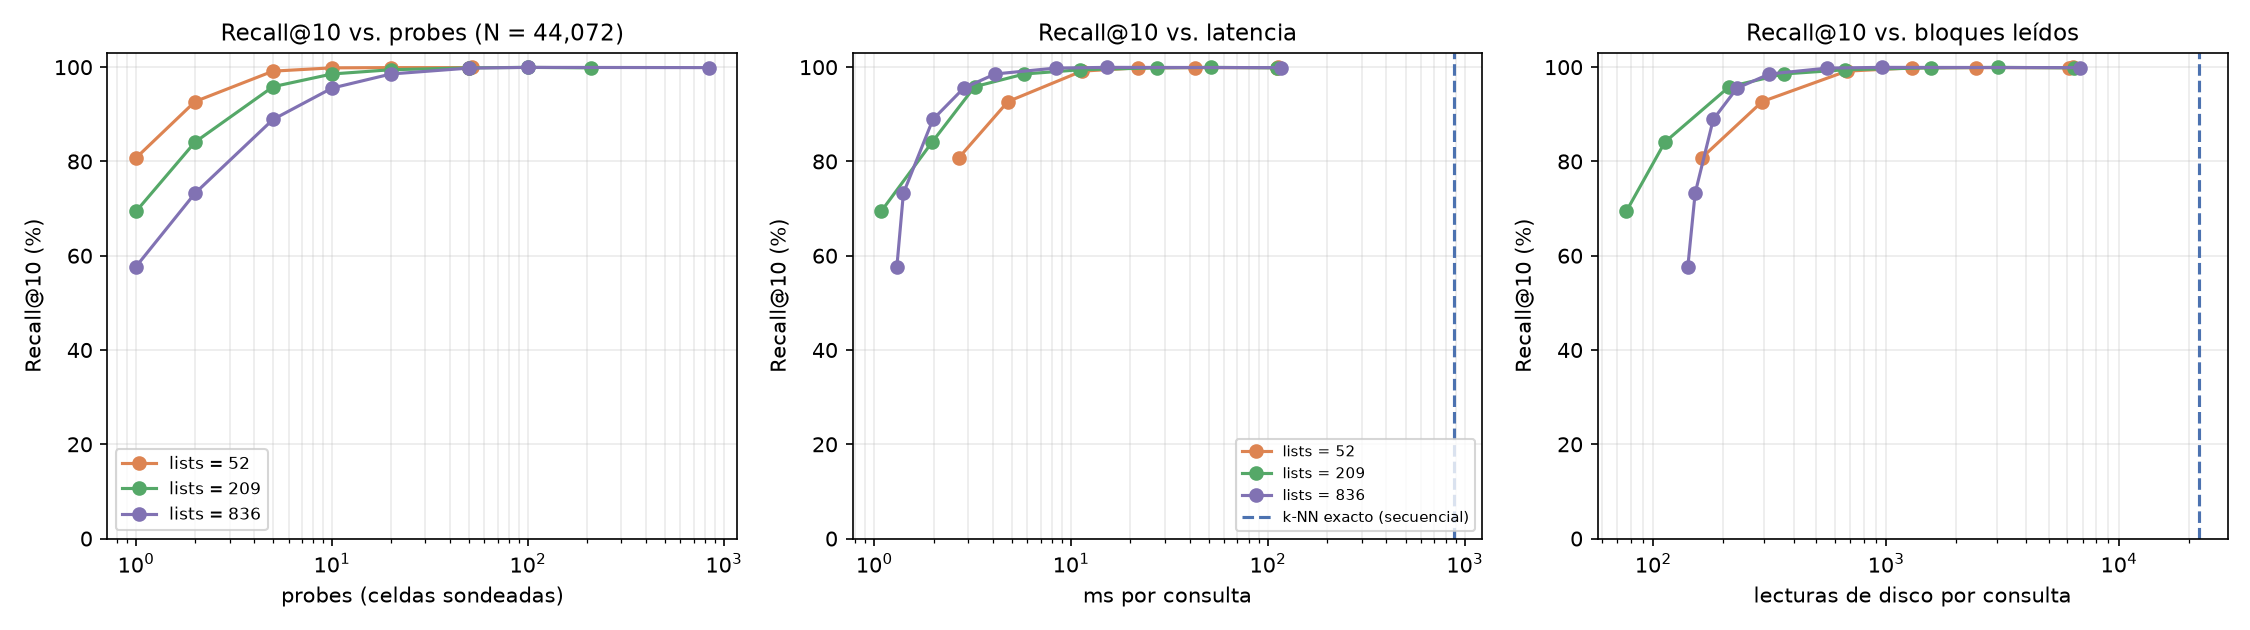
\includegraphics[width=\textwidth]{exp8_recall.png}
\caption{Experimento 8: curvas de compromiso entre Recall@10, \code{probes}, latencia y bloques
leídos. La línea vertical es el $k$-NN exacto por recorrido secuencial.}
\label{fig:exp8}
\end{figure}

\paragraph{Análisis.}
\begin{itemize}
\item \textbf{El compromiso}: con $C=\sqrt N=209$ celdas, \code{probes} = 1 compara solo el 0.6\,\%
  de los vectores y ya encuentra el 69\,\% de los vecinos verdaderos; con \code{probes} = 5 el
  recall es 95.9\,\% (212 bloques, 3.2\,ms) y con \code{probes} = 10, 98.6\,\% (363 bloques,
  5.8\,ms). El $k$-NN exacto lee 22\,036 bloques y tarda 879\,ms: el IVF con \code{probes} = 10 lee
  el \textbf{1.6\,\%} de los bloques y es \textbf{150 veces más rápido} a cambio de perder 1.4 puntos
  de recall. El recall crece de forma cóncava: cada celda adicional aporta menos vecinos nuevos.
\item \textbf{El costo sigue la fórmula}: las lecturas son las páginas del directorio
  ($\lceil C/7\rceil$ = 30 con $C=209$) más las de las celdas sondeadas ($\approx$\,probes\,$\cdot
  N/(7C)$ = 30 por celda) más los 10 registros: con \code{probes} = 5, $30+151+10\approx$ 191
  estimadas y 212 medidas (las celdas cercanas a la consulta son más densas que el promedio).
\item \textbf{Número de celdas}: con pocas celdas ($C=52$) cada una es grande: \code{probes} = 1 ya
  da 80.8\,\% de recall, pero leyendo 161 bloques. Con muchas ($C=836$) las celdas son pequeñas y se
  alcanza el mismo recall comparando menos vectores (98.6\,\% con el 2.8\,\% de los vectores, frente
  al 5.1\,\% con $C=209$), pero el directorio crece (120 páginas que se leen en cada consulta) y
  domina cuando \code{probes} es pequeño. En bloques leídos para un recall de $\approx$98.6\,\%:
  315 con $C=836$ frente a 363 con $C=209$; con $C=52$ hacen falta 676 para llegar al 99.2\,\%. $C=\sqrt N$ es un buen punto
  medio; con más celdas convendría mantener los centroides en memoria.
\item \textbf{Exactitud en el límite}: con \code{probes} $=C$ se comparan todos los vectores; el
  recall medido es 99.9\,\% y no 100\,\% porque el catálogo tiene imágenes duplicadas con el mismo
  \emph{embedding} y los empates en la posición 10 se resuelven distinto que en la verdad base.
  Incluso así el IVF exhaustivo lee 6\,425 bloques frente a 22\,036, porque sus páginas solo guardan
  $\langle\text{RID}, \vec v\rangle$ (7 por página) y la tabla guarda registros de 1\,708 bytes (2 por
  página).
\end{itemize}


%==========================================================================================
\section{Pruebas}

A las 133 pruebas del Entregable~1 se suman 56: \code{test\_rtree.py} (capacidades desde $B$;
invariantes tras miles de inserciones: contención de cajas, profundidad uniforme, número de entradas;
ventana, radio y $k$-NN contra fuerza bruta; STR; borrado; persistencia; dimensiones altas),
\code{test\_inverted\_index.py} (analizadores; mezclas con dos punteros; SPIMI con varios bloques
contra un solo bloque; listas ordenadas; lectura exclusiva de las páginas del término; ranking contra
un modelo TF-IDF en memoria con tolerancia $10^{-6}$; consultas booleanas; BM25; BoVW;
reconstrucción), \code{test\_ivf.py} (K-Means; reparto de todos los vectores; exactitud con
\code{probes} $=C$; recall e I/O crecientes con \code{probes}; inserción y borrado; persistencia) y
\code{test\_multimodal.py}, que ejecuta por SQL las mismas consultas sobre una base sin índices y
otra con índices y exige resultados idénticos, además de verificar la estrategia elegida, el
desglose de I/O y los errores. En total, 189 pruebas.

%==========================================================================================
\section{Decisiones y limitaciones}

\begin{itemize}
\item \textbf{Registros de longitud fija.} \code{TEXT(n)} y \code{VECTOR(n)} reservan su tamaño
  máximo y el registro debe caber en una página; a cambio el RID sigue siendo estable y el acceso por
  RID cuesta una lectura. Documentos más largos requerirían páginas ranuradas o un archivo de
  \emph{blobs}.
\item \textbf{Índice invertido estático}: las actualizaciones lo marcan como desactualizado y se
  reconstruye antes de la siguiente búsqueda. Adecuado para cargas masivas seguidas de consultas.
\item \textbf{Sin \emph{buffer pool}}: el directorio del IVF y el diccionario se leen en cada
  consulta, de modo que el I/O informado es el real.
\item \textbf{R-Tree sin condensación} en el borrado y \textbf{IVF sin reentrenamiento} automático
  (salvo el de un índice creado sobre una tabla vacía).
\item \textbf{Estimación de selectividad} con valores por defecto para predicados espaciales y
  textuales; un histograma por columna mejoraría la elección entre pre y post-filtering.
\item \textbf{Aritmética con \code{numpy}} sobre páginas ya leídas; el almacenamiento sigue siendo
  una página por transferencia a través de \code{DiskManager}.
\end{itemize}

%==========================================================================================
\section{Conclusiones}

\begin{itemize}
\item \textbf{El mismo principio en tres dominios}: R-Tree, índice invertido e IVF hacen lo mismo que
  el B$^+$ y el hash del Entregable~1: organizar las páginas para leer solo las que pueden contener la
  respuesta. Midiendo bloques, un $k$-NN geográfico pasa de 1\,235 lecturas a 12, un Top-10 textual
  de 2\,320 a 128--252 y un $k$-NN vectorial de 22\,036 a 363 (con 98.6\,\% de recall).
\item \textbf{Los índices no agrupados pagan por fila}: tanto el R-Tree por radio como las consultas
  booleanas poco selectivas leen más bloques que un recorrido secuencial cuando califican más filas
  que páginas tiene la tabla. Las consultas con ranking y \code{LIMIT} no tienen ese problema porque
  solo traen $K$ registros.
\item \textbf{La dimensión decide la estructura}: el R-Tree deja de servir a partir de $D\approx16$
  (visita el 99\,\% de sus hojas); para los vectores de 128 dimensiones hay que renunciar a la
  exactitud, y el IVF convierte esa renuncia en un parámetro (\code{probes}).
\item \textbf{Guardar lo necesario para puntuar}: tener $tf$ en los posteos y la norma precalculada
  hace que nuestro ranking Top-10 sea unas 30 veces más rápido que \code{ts\_rank} sobre GIN, aunque
  PostgreSQL sea mucho más rápido en las consultas booleanas.
\item \textbf{Los \emph{embeddings} superan al BoVW} en efectividad (P@10 0.79 frente a 0.51), en
  latencia (6\,ms frente a 134\,ms) y en bloques leídos, con el mismo costo de extracción.
\item \textbf{Ninguna estrategia híbrida es siempre mejor}: con un filtro que deja pasar el 79\,\% de
  las filas el \emph{post-filtering} lee 223 bloques y el \emph{pre-filtering} 34\,822; con uno que
  deja pasar el 0.5\,\% el \emph{pre-filtering} lee 208 y el \emph{post-filtering} ni siquiera
  completa los $k$ resultados. Estimar el costo de ambas y elegir es indispensable.
\end{itemize}

\paragraph{Trabajo futuro.} Índice invertido incremental (segmentos y fusión), compresión de las
listas de posteo, HNSW en disco, cuantización de producto para el IVF, histogramas para estimar la
selectividad y un \emph{buffer pool} para el directorio de centroides y el diccionario.


\begin{thebibliography}{9}
\bibitem{guttman} A. Guttman. R-trees: a dynamic index structure for spatial searching. \emph{SIGMOD}, 1984.
\bibitem{str} S. Leutenegger, M. López y J. Edgington. STR: a simple and efficient algorithm for R-tree packing. \emph{ICDE}, 1997.
\bibitem{hjaltason} G. Hjaltason y H. Samet. Distance browsing in spatial databases. \emph{ACM TODS}, 24(2):265--318, 1999.
\bibitem{manning} C. Manning, P. Raghavan y H. Schütze. \emph{Introduction to Information Retrieval}. Cambridge University Press, 2008.
\bibitem{sivic} J. Sivic y A. Zisserman. Video Google: a text retrieval approach to object matching in videos. \emph{ICCV}, 2003.
\bibitem{lowe} D. Lowe. Distinctive image features from scale-invariant keypoints. \emph{IJCV}, 60(2):91--110, 2004.
\bibitem{he} K. He, X. Zhang, S. Ren y J. Sun. Deep residual learning for image recognition. \emph{CVPR}, 2016.
\bibitem{jegou} H. Jégou, M. Douze y C. Schmid. Product quantization for nearest neighbor search. \emph{IEEE TPAMI}, 33(1):117--128, 2011.
\bibitem{ramakrishnan} R. Ramakrishnan y J. Gehrke. \emph{Database Management Systems}, 3.\textsuperscript{a} ed. McGraw-Hill, 2003.
\end{thebibliography}

\end{document}
